% 独自のコマンド

% ■ アブストラクト
%  \begin{jabstract} 〜 \end{jabstract}  :日本語のアブストラクト
%  \begin{eabstract} 〜 \end{eabstract}  :英語のアブストラクト

% ■ 謝辞
%  \begin{acknowledgment} 〜 \end{acknowledgment}

% ■ 文献リスト
%  \begin{bib}[100] 〜 \end{bib}


\newif\ifjapanese

\japanesetrue  % 論文全体を日本語で書く(英語で書くならコメントアウト)

\ifjapanese
  \documentclass[a4j,twoside,openright,11pt]{jreport} % 両面印刷の場合。余白を綴じ側に作って右起こし。
  % \usepackage[backend=bibtex]{biblatex}
  %\documentclass[a4j,11pt]{jreport}                  % 片面印刷の場合。
  \renewcommand{\bibname}{参考文献}
  \newcommand{\acknowledgmentname}{謝辞}
\else
  \documentclass[a4paper,11pt]{report}
  \newcommand{\acknowledgmentname}{Acknowledgment}
\fi
\usepackage{thesis}
\usepackage{ascmac}
\usepackage[dvipdfmx]{graphicx}
\usepackage{multirow}
\usepackage{url}
\usepackage{lscape}
\usepackage{listings}
%\bibliographystyle{jplain}
\bibliographystyle{junsrt}

\bindermode  % バインダー用余白設定

% 日本語情報(必要なら)
\jclass  {卒業論文}                             % 論文種別
\jtitle    {ユーザインタフェースの設計をサポートするノーデザインツールの研究}    % タイトル。改行する場合は\\を入れる
\juniv    {慶應義塾大学}                  % 大学名
\jfaculty  {環境情報学部}               % 学部、学科
\jauthor  {尾崎 正和}                       % 著者
\jhyear  {3}                                   % 平成○年度
\jsyear  {2021}                                 % 西暦○年度
\jkeyword  {UI, ノーデザイン, ノーコード, プロダクト開発, UI自動生成, インターフェースビルダー, 人間中心設計}     % 論文のキーワード
\jproject{全世界インタフェースデザイン (増井研究会)} %プロジェクト名
\jdate{2022年1月}

% 英語情報(必要なら)
\eclass  {Graduation Thesis}                            % 論文種別
\etitle    {Research on the realization of "no-design" tools that go beyond no-codes}      % タイトル。改行する場合は\\を入れる
\euniv  {Keio University}                             % 大学名
\efaculty  {Faculty of Environment and Information Studies}  % 学部、学科
\eauthor  {Masakaz Ozaki}                           % 著者
\eyear  {2021}                                        % 西暦○年度
\ekeyword  { User Interface, No-design, No-code, Product Development, UI Generation, Interface Builder, Human Centered Design }          % 論文のキーワード
\eproject{Masui Lab}                 %プロジェクト名
\edate{January 2022}





\begin{document}

\ifjapanese
  \jmaketitle    % 表紙(日本語)
\else
  \emaketitle    % 表紙(英語)
\fi


\begin{jabstract}

スマートフォンやパーソナルコンピュータの急激な普及につれ,様々な応用ソフト(アプリケーション)が開発され人々が毎日利用している.近年ではアプリケーション開発において十分な開発時間,人員,技術が確保することが難しく質の担保されたアプリケーションを設計し開発することが難しくなっている.そして個人開発者,スタートアップ企業,アイディアはあるが実装する力のない個人などではさらにこれを行うことが難しくなる.

その流れに伴い「ノーコード」と呼ばれるプログラミングやコンピュータサイエンスに精通していない人でも簡単にアプリケーションを開発できるサービスが登場した.しかしながら現在のノーコードにおいてもアプリケーションのユーザインタフェースデザインはユーザが行うか,テンプレートを利用する他ないためユーザインタフェースに精通していないユーザでは自由度の高く質の担保されたユーザインタフェースのアプリケーションを開発するのは困難である.

そこで本研究では,本来大規模な開発でしか行われない専門のユーザインタフェースデザインを自動化し,ユーザインタフェースに関する専門的な知識がなくても容易にユーザインタフェースを開発できるようにするためのシステムの開発をおこなった.ユーザインタフェースの設計の方法については確立された手法はなくデザイナのセンスと経験に委ねられていた部分が多かったが,既存のユーザインタフェースを分析していくことでユーザインタフェースは画面に表示されている要素の数と種類,各要素のグルーピング,画面内での要素がもつ優先度が決定されればインターフェースを制作できるのではないかという仮説を立てた.その仮説に基づきiOS向けのネイティブアプリケーションのユーザインタフェースを専門的知識なしに制作できるシステムを開発し有用性を明らかにした.
\end{jabstract}


\begin{eabstract}
High-quality, easy-to-use UI design requires in-depth professional knowledge and experience.
We will propose a system that builds UI automatically.  Our system enables designing UI without professional knowledge and experience.

There is no established method for UI design.
So, it has often been left to the sense and experience of the designer. 

    However, the UI of smartphone applications is similar and has not changed significantly for decades. 
Hence, we thought that there must be some kind of rule.

By analyzing existing interfaces, we hypothesized that  UI can be built if the number and types of elements, the grouping of each element, and the priority of each element are determined.
Also, in general, when we talk about "design" in software, we tend to focus on the appearance of the interface.

By automating the appearance of interfaces, a designer can focus on the essential design. 
 Based on this hypothesis, we developed a system that allows users to generate user interface source codes for native iOS applications (SwiftUI) without specialized knowledge.  
After that, evaluated the usefulness of this system.

\end{eabstract}
  % アブストラクト。要独自コマンド、include先参照のこと

\tableofcontents  % 目次
\listoffigures    % 表目次
\listoftables    % 図目次

\pagenumbering{arabic}

\chapter{序論}
\label{chap:introduction}

\section{背景}

近年,スマートフォンの急速な普及により数多くのアプリケーションが開発され,人々が毎日利用している,そのアプリケーションの開発には人々が感じている課題の洗い出し,適切な仕様の確定,使いやすいインタフェースの設計,実装など専門的で複雑な工程が多数存在する.中でもインタフェース設計とその実装は開発全体の中で設計段階で45%,実装段階で50%,保守段階で37%の時間を占めると言われている\cite{myers1992survey}.

またデザインカンパニーであるGoodpatchの社長である土屋は創業の原点について次のように述べており,デザインの重要性について述べている.

\begin{quotation}
Goodpatchは2011年にUIデザインに特化したデザイン会社としてスタートしました。2011年に起業前に渡ったサンフランシスコでは創業期のInstagramやUber、Airbnbなど多くのスタートアップの共同創業者にデザイナーがおり、ベータ版からUIデザインに力を入れ、ユーザー体験を最初から考え、デザインを重要な差別化要素としてプロダクト開発を行っておりました。日本の環境と大きなギャップを感じた土屋は日本に帰り、創業したことがGoodpatchの原点です。\cite{goodpatchwhydesign}
\end{quotation}

大手企業の大規模開発では社内に専門知識を持ったデザイナが在籍していたり,Goodpatchのようなデザインカンパニーと共に設計を行うことが可能であるが専門のデザイナが在籍しないスタートアップ企業やインディーズ開発,個人開発ではこれらを行うのは非常に困難である.

また,日本ではデザインが装飾などの表層的なもののみを指すと誤解されていると指摘されている\cite{goodpatchwhydesign}.本来のデザインの役割とは,本質的な(何の?)価値を見出し,価値を最大化させることである.GarretのUX五段階モデル(図\ref{fig:garretuxmodel})は,具象と抽象を行き来しながら,戦略,要件,構造,骨格,表層全てを設計することがデザインであると示している.

\begin{figure}[htbp]
  \begin{minipage}{\hsize}
    \begin{center}
       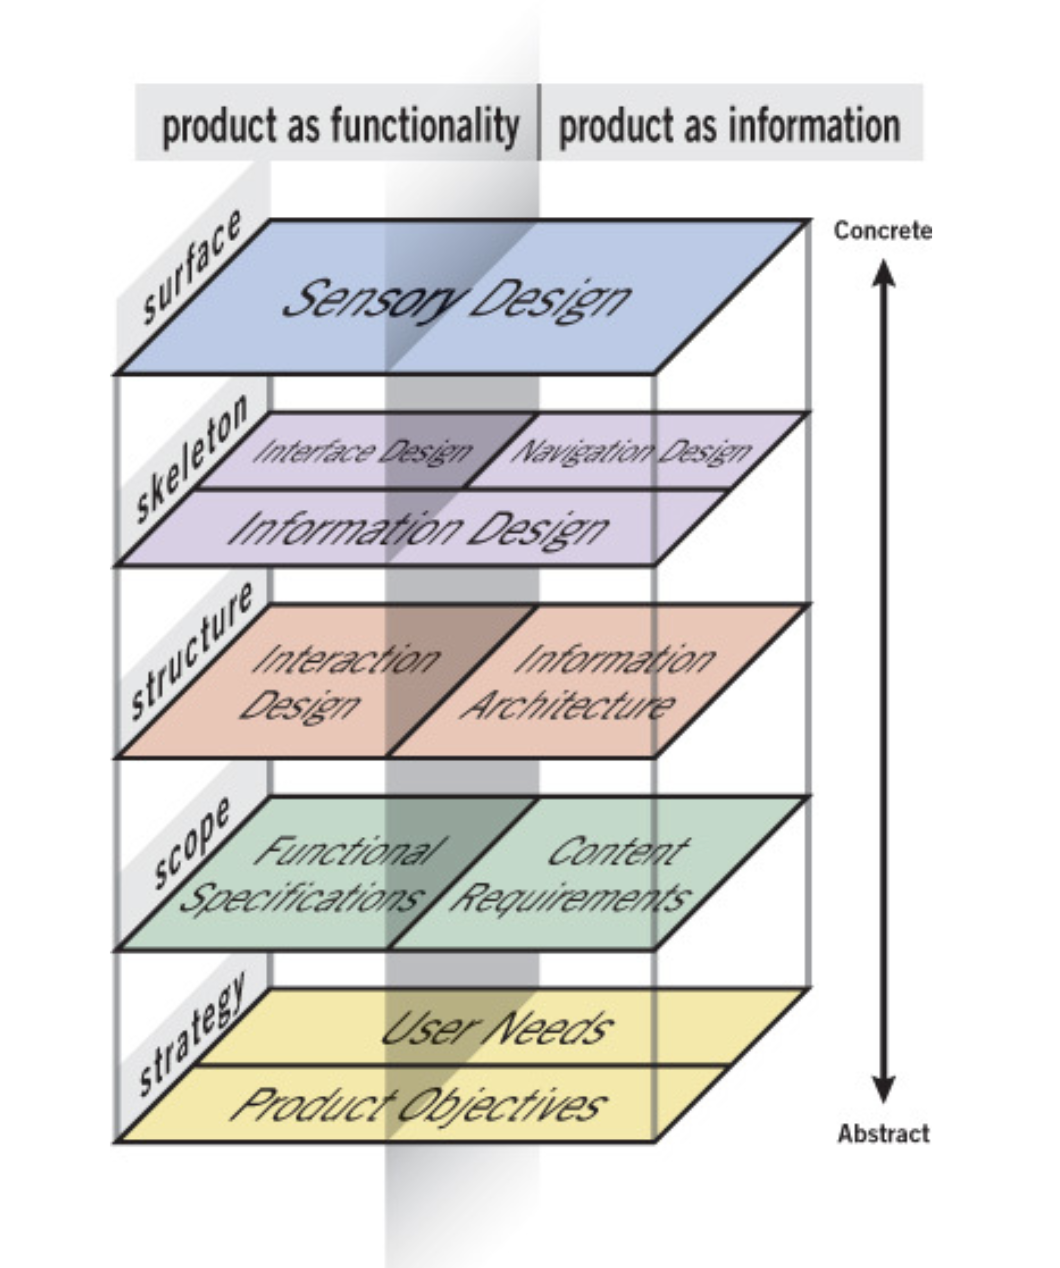
\includegraphics[width=100mm]{img/uxmodel.png}
    \end{center}
    \caption{GarretのUX五段階モデル\cite{garrett2010elements}}
    \label{fig:garretuxmodel}
  \end{minipage}
\end{figure}

%サブセクションが内容を表していなかったので変えた
\subsection{システム開発におけるデザイナの役割と現状}

%↓尾崎氏の個人的意見になっているので客観的に

資金や人的リソースが十分な大規模開発では役割としてのデザイナが参画している場合も多いが,前述のようなデザインの能力を有しているとは限らない.職業としてのデザイナを職業としている人の中でもGarretが述べている本来のデザインを忘れ,表層のデザインに注力してる場合が多く本来のデザインが一般に普及しているとは言えない.(←ソースは?

また,デザイナよりもアプリに向き合っている時間が長いエンジニアの方がアプリのデザインについて専門的知識を持ち開発をおこなっている場合も多数ある.エンジニアの場合GarretのUX五段階モデルもさることながら,UIが実際に動く仕組みを理解している分,内部構造という面での専門知識を有してる場合も多い.
実際に日本経済新聞電子版のメンバーによるデザインに関する登壇では14個中全ての登壇がエンジニア,又はエンジニア経験のある人の登壇となっている.\cite{nikkeislide}

個人開発アプリは大規模開発するほど収益が見込まれないものの,ニッチな消費者のニーズにあうさまざまなアプリケーションがアプリストアにリリースされている.しかしながら資金,時間,人的リソースが十分にない個人開発では開発者がデザインの重要性について理解した専門家がいないことにより使い勝手が悪いものや,表層のデザインにのみ注力したアプリケーションがあり,消費者のニーズに答えられずにいる.

%以上のことから下の(1)(2)が導かれていない.上で言っているのはエンジニアが専門知識を有しているので大規模開発ではエンジニアがデザインをすればいい,個人開発では専門家が居ないと言っているだけなので(1)を導くには飛躍しすぎている.

%(2)については奥深くのデザインが何なのかわからない.

以上のことから,(1)現在は大規模な開発でしか行われていない専門性の高いユーザインタフェースデザインのハードルを下げること,(2)表層のデザインにとらわれずに奥深くのデザインに注力することができる手法を開発することが求められる.

\section{目的}
本研究では(1)現在は大規模な開発でしか行われていない専門性の高いユーザインタフェースデザインのハードルを下げ,(2) 表層のデザインにとらわれずに奥深くのデザインに注力することができるようにするシステムの開発を目指す.

%↓本当か?設計手法はいくつかあるのでは?OOUIとか.それらの不満点を示す必要がある.UI設計の手法を確立すれば自動生成できるというのはおかしくない?別の話では?「本来のデザイン」がよくわからない.

現在のUIデザインには確立された設計手法はなく,デザイナの経験やセンスに頼っているものの,既存のUIを分析することによりUI設計の手法を確立すれば簡易なUI自動生成システムになり得る.また,(2)注力されがちであった表層のデザインを自動化することでデザイナ,個人開発者が本来のデザインに向き合うことにも目を自然と向けられるようになることが可能になる.

本研究ではこの手法になりうる仮説として,1画面に必要な要素一覧,各要素の相対的な優先度,要素同士のグルーピングからUIを自動で生成する手法を提案する.%ここでノーデザインという言葉を主張していく

そして提案した手法をもとに1画面に必要な要素一覧,各要素の相対的な優先度,要素同士のグルーピングの情報からiOSネイティブアプリケーションのソースコード(SwiftUI)を自動で生成するシステムを開発した.そして,開発したシステムの有用性を示した.

\section{本論文の構成}

本論文の構成を示す.

第\ref{chap:introduction}章では本研究の背景について述べた.第\ref{chap:prevresearch}章では関連研究と諸概念を整理する.第\ref{chap:pulsewave}章では要素,優先度,グルーピングからUIを自動生成する手法を提案し,第\ref{chap:pulsewave}章ではその手法をもとにiOS向けネイティブアプリケーションのコードを生成するシステムを提案する.そして,それらの有効性を示す.最後に,第\ref{chap:conclusion}章の結論では本研究を総括し,考察と展望を述べる.付録として,本研究で行った実験で得られたデータを添付する.
  % 本文1
%軽く最後に書く.2章には持ってこない.
\chapter{関連研究と諸概念の整理}
\label{chap:prevresearch}

\section{ユーザインタフェースのデザイン手法}

%なんか内容がびみょういな.知りたいのはそういうことではない
%今UIデザインは大変だ 配置とかが大変だ
\subsection{大規模開発に置けるユーザインタフェースデザイン}
\subsection{個人開発に置けるユーザインタフェースデザイン}

\section{ノーコードでのシステム開発}
大規模な開発を行うリソースがない企業や専門知識をあまり持たない個人でもアプリケーションやウェブサイトを作れるように近年,ノーコードと呼ばれるサービスが登場した.ノーコードとは文字通り,コーディングを行わずにアプリケーションやウェブサイトを作れるサービスである.

全体を通して,コードを書かないのでコードを書けばできることができない.


ここでは既存のノーコードのサービスの例をいくつかあげ,特徴と課題点を挙げていく.
\subsection{STUDIO}
STUDIOはSTUDIO株式会社が運営する

デザインの自由度が高いのがウリ.自由度の高いノーコードってイラレみたいで結局表層のビジュアルデザインに目を向けがち.
web front-endの専門知識はなくても行えるが,デザインの専門知識は求められる.
自由度の高いビジュアルデザインを売りにしているが,細かなインタラクションなどを追加でソースコードを書くことで補えないのでSTUDIOのできる範囲内で行わなければならない.
素人ではなくある程度知識のある人が使うものであるにもかかわらず,STUDIOで制作したwebサイトは一目でわかってしまうため,コードを書けないと自分で宣言しているようなものである.

\subsection{Glide}
Google Spread Sheetsなどをデータベースとして扱い,テンプレートベースの簡易なアプリを作れる.
スケーラビリティが終わっている
テンプレートベース
社内ツールの自動化や小規模のもの向けでこれで作ったものをプロダクトとして出すことは難しい


\subsection{Microsoft Power Apps}
Glideと同じような感じであるが,若干のスケーラビリティがる.
同じくビジネスツールなのでそれ自体をプロダクトにすることは難しい

\section{デザインの自動化}
デザインの専門知識がない人でもテンプレートに頼らず適切のUIを制作できるようにUIの自動生成を行う研究が行われている
\subsection{機械学習を用いたUIの自動生成}
機械学習使うと次同じインプットでやった時にも同じのが出てくると限らないので適していない
\subsubsection{GANを用いた自動生成}

\subsubsection{GPT-3を用いた自動生成}

\section{問題の所在}

\begin{itemize}
	\item デザインを表層のデザインだけだと誤解している %表層のデザインしかしないシステムを作るので言葉が足りない
	\item 既存のノーコードではデザインは自分で行う又はテンプレートから選んだデザインをそのまま使用する必要がある
	\item 機械学習を用いた自動生成では一意性が担保できない.
	\item GANで生成したUIは画像なのでアプリとして機能しない.
\end{itemize}
また,スマートフォンのUIは2007年の初代iPhoneから,パソコンについては1984年の初代Macintoshから基本的なUIは全く変わっていないにもかかわらず,UIの生成の法則性の研究はあまり行われてこなかった.


以上のことから表層のデザインを自動化し,専門知識のない人でも
  % 本文2
\chapter{ノーデザイン: 要素,優先度,グルーピングの情報からのUI自動生成手法の提案}
\label{chap:auto-gen}

本章では,後述のiOSネイティブアプリケーションのインタフェース自動生成システムの開発に先立ち,既存のインタフェースの分析から導きさした要素,優先度,グルーピングによりインタフェースの構築が行える法則について検討した.自動生成を行うアルゴリズムの提案行う.
\section{既存インタフェースの分析}
既存のiOSネイティブアプリケーションのUIの分析をおこなっていく.
画面内でのUIは画面遷移を司り,画面内の体験には直接影響を与えないものが存在する.
わかりやすくするために,画面遷移を司るUIとそうでないUIについて分類して考えていく.
\subsection{画面遷移を司るUI}
HIGのhierarchical Navigation,
FlatNavigation
Content-Driven or Experience-Driven Navigation
大体こうなってる.


今回の自動生成手法の提案ではこのような画面遷移を司るUIは切り離し,画面内のコンテンツのUIに注目して考えいく.
実際のSwiftUIのコードでも画面遷移を司るUIとコンテンツは別で実装されて画面遷移の上にコンテンツが乗る形式になる.のでこの方針は問題ない



\subsection{要素}
画面内に何を置くかは考える必要がある
要素をマーキングしたスクショを何枚か載せる
\subsection{優先度}
優先度がありそうだ.
優先度も考えたダイアグラムを何枚か載せる
\subsection{グルーピング}
グルーピングのダイアグラムを何枚か載せる
グルーピングがありそうだとのべる

\section{アルゴリズムの構築}
要素を優先度の高い順に画面内に縦に並べていくのが基本.
グループは一つの要素としてカウントする.(優先度は中の要素の優先度の足し合わせ)
要素の中にはユーザが操作するもの,見るだけのものがあり,操作するものは全体に並ぶと良い.
Groupが入れ子になる場合はHstack, Vstackを交互にすることによって大体のUIを構成できる.
画面内の要素の優先度の基準を10とし,それを超える場合はスクロールするようにする.
これで大体いい感じになる.Padding等は適切につけていく.
優先度が上がる度に文字は大きく,太く,ボタンもただの青文字ではなく,borderがついたり,塗り領域が増えたりとしていく.

  % 本文3
\chapter{iOSネイティブアプリケーションのインタフェース自動生成システムの開発}
\label{chap:impl}
前述の既存UIの分析と分析から導き出したアルゴリズムをもとにiOSのネイティブアプリケーションのインタフェース自動生成システムの開発を行った.

また,本自動生成システムを用いて既存UIの再生成をおこなった他,普段からiOSのネイティブアプリケーションを個人開発している14-17歳の男女を被験者とした本システムの有用性をはかる実験を行い,有用性を示すことができた.

本システムの設計は以下のとおりである.
\section{システムの設計・開発}
要素,優先度,グルーピング情報からの画面のコンテンツUI自動生成システムのプロトタイプとして主要な部分のみを実装した.本研究において画面のコンテンツUIとは実際画面に表示されるUIのうち,画面遷移を司どるUI,画面のタイトル表示を除いたものを指す.

本研究のUI自動生成において重要なのは画面内の要素,優先度,グルーピング,の情報のみでUIを自動生成できることである.この点を実現するためのシステムを開発した.

本システムで利用できる要素(UIパーツ)の名称と機能は以下(表\ref{table:ui_elements})とする.名称の命名に関しては基本的にSwiftUIでの名称を使用するが,SwiftUIではテキスト表示の行数による名称の違いがないため独自に一行表示をLabel, 複数行表示をTextViewとした.
\begin{landscape}
\begin{table}[htbp]
\centering
\scalebox{1.0}{
\begin{tabular}{llllllllllllllll}
\hline
本システムでの名称                    &UIKitでの名称                    &SwiftUIでの名称                      &ユーザの操作の有無                      &主な使用用途 \\ \hline
Label &UILabel                            & Text                                     &無                                                    & 一行の文字列を表示するために使用する\\
TextView &UITextView                      & Text                                     &場合によっては有                               & 複数行の文字列を表示, 入力, 編集するのに使用する\\
TextField &UITextField                      & TextField                              &有                                                    & 一行の文字を入力するために使用する\\
Button &UIButton                          & Button                                  &有                                                    & タップアクションを取得するために使用する \\
Toggle &UISwitch                          & Toggle                                  &有                                                    & ON/OFFの切り替えのために使用する \\
Image &UIImageVIew                   & Image                                   &無                                                    & 画像表示のために使用する\\
Map &MKMapView                    & Map                                     &有                                                    & 地図の表示のために使用する\\
DatePicker &UIDatePicker                   & DatePicker                            &有                                                    & 日付選択のために使用する\\
Slider &UISlider                           & Slider                                    &有                                                    & 特定の数値を調整するために使用する\\ \hline
\end{tabular}
}
\caption{利用可能な要素一覧}
\label{table:ui_elements}
\end{table}
\end{landscape}
\subsection{基本的な配置アルゴリズム}
前述のアルゴリズムより,基本的には要素を優先度順に縦に配置する.グループも一要素として扱い表示を行う.グループ内のレイアウトについては後述のグルーピングセクションで行う.

基本的な優先度に加え,UIの要素にはユーザからの操作を受け付けるものと受け付けないものがある.ユーザからの操作を受け付けるものに関しては指の届きやすい画面下に配置するのが適切であり,以下の表\ref{table:viewArrangementRatio}のように各要素の種類ごとに配置係数を定め,後述の優先度の値と掛け合わせた値の昇順に配置する.
\begin{table}[htbp]
\centering
\scalebox{1.0}{
\begin{tabular}{llllllllllllllll}
\hline
名称                    &配置係数 \\ \hline
Label                   &1.0\\
TextView             &0.9\\
TextField             &0.8\\
Button                 &0.5\\
Toggle                 &0.5\\
Image                  &2.0\\
Map                    &1.5\\
DatePicker          &0.7\\
Slider                  &0.7\\ \hline
\end{tabular}
}
\caption{各要素の配置係数}
\label{table:viewArrangementRatio}
\end{table}

\subsection{優先度}
本システムにおいて優先度からは要素の視覚的な目立たせ具合,表示順序を決定する.
優先度の値は一画面あたりの合計を10とし,それを超えた場合はスクロールする画面が提供される.
優先度による各要素の目立たせ具合は以下の通りである.以後登場するスクリーンショットは全て本システムによって自動生成されたUIである.


\subsubsection{Label}
図\ref{fig:label_priority}のように優先度ごとに文字の大きさ,太さを調整して実装した.優先度5以上でもこれ以上の大きさになることはなく,それ以上の優先度は配置にのみ反映されるようにした.

\begin{figure}[htbp]
  \begin{minipage}{\hsize}
    \begin{center}
       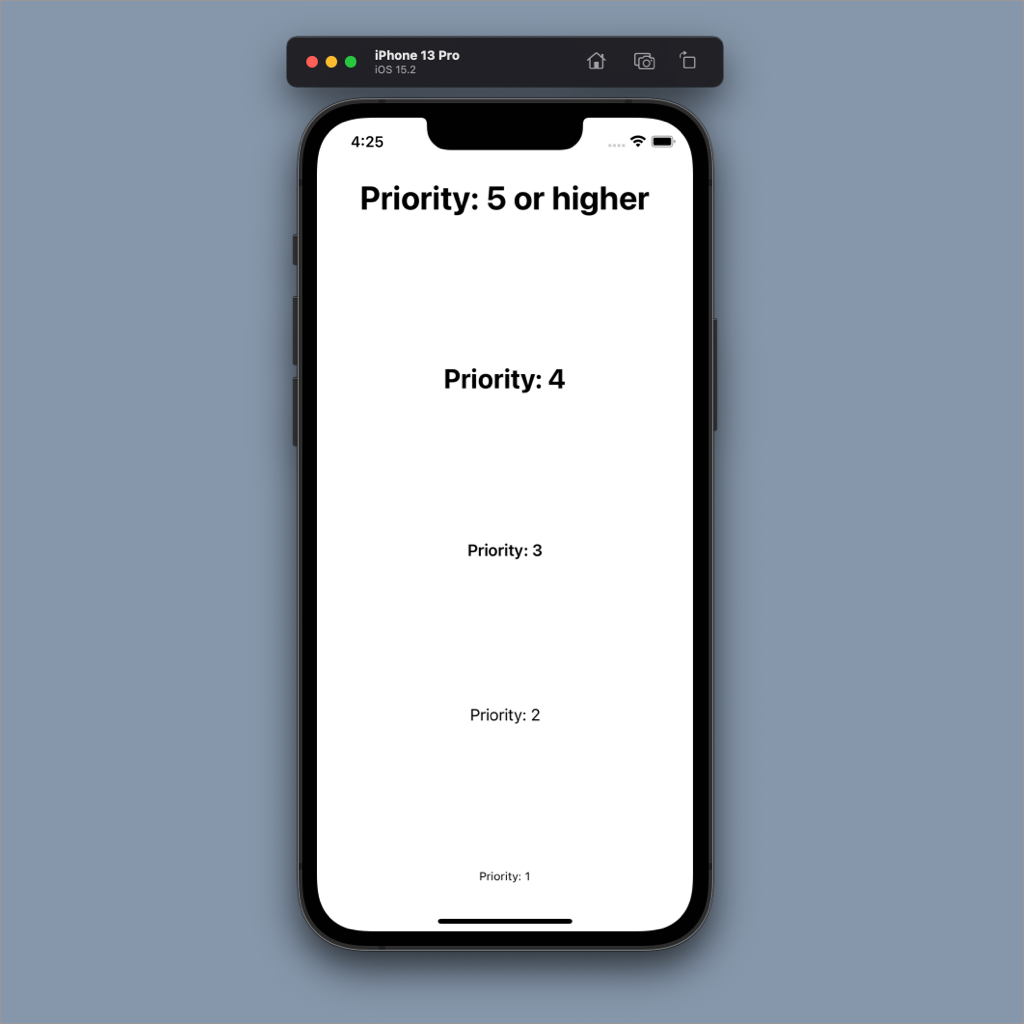
\includegraphics[width=100mm]{img/Label_priority.png}
    \end{center}
    \caption{Labelの優先度による視覚的目立たせ具合}
    \label{fig:label_priority}
  \end{minipage}
\end{figure}

\subsubsection{TextView}
図\ref{fig:TextView_priority}のように実装した.前述のLabelから文字の太さ,大きさを少し調整すると共に,最大行の指定を優先度1の場合は2行まで, 優先度2の場合は4行まで,優先度3の場合は5行まで,優先度4の場合は8行まで,優先度5以上の場合は15行を最大とした.優先度5以上でもこれ以上の大きさになることはなく,配置のみに優先度を利用する.

\begin{figure}[htbp]
  \begin{minipage}{\hsize}
    \begin{center}
       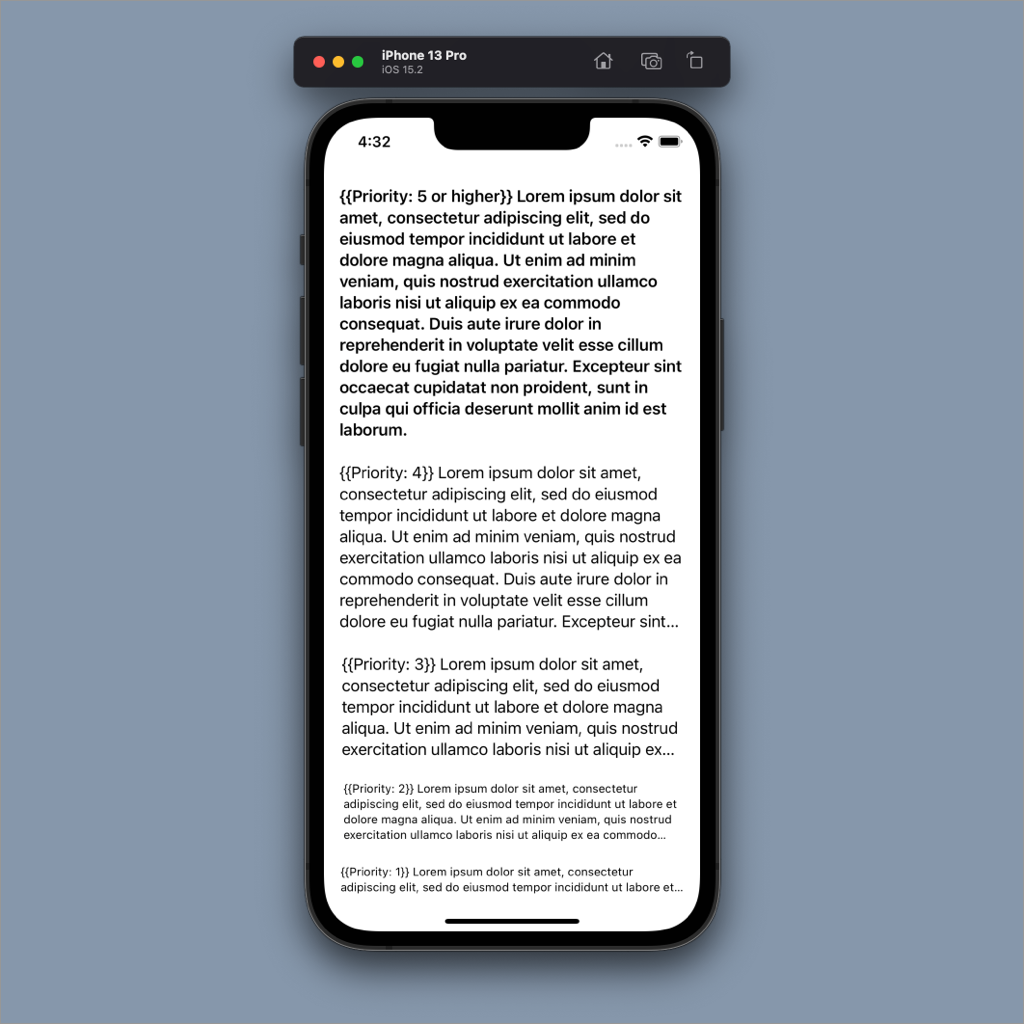
\includegraphics[width=100mm]{img/TextView_priority.png}
    \end{center}
    \caption{TextViewの優先度による視覚的目立たせ具合}
    \label{fig:TextView_priority}
  \end{minipage}
\end{figure}

\subsubsection{Button}
図\ref{fig:button_priority}のように実装した.優先度によって文字の大きさ,文字の太さ,タップエリアの大きさ,色等が変更されている.優先度5以上でもこれ以上の大きさになることはなく,配置のみに優先度を利用する.
\begin{figure}[htbp]
  \begin{minipage}{\hsize}
    \begin{center}
       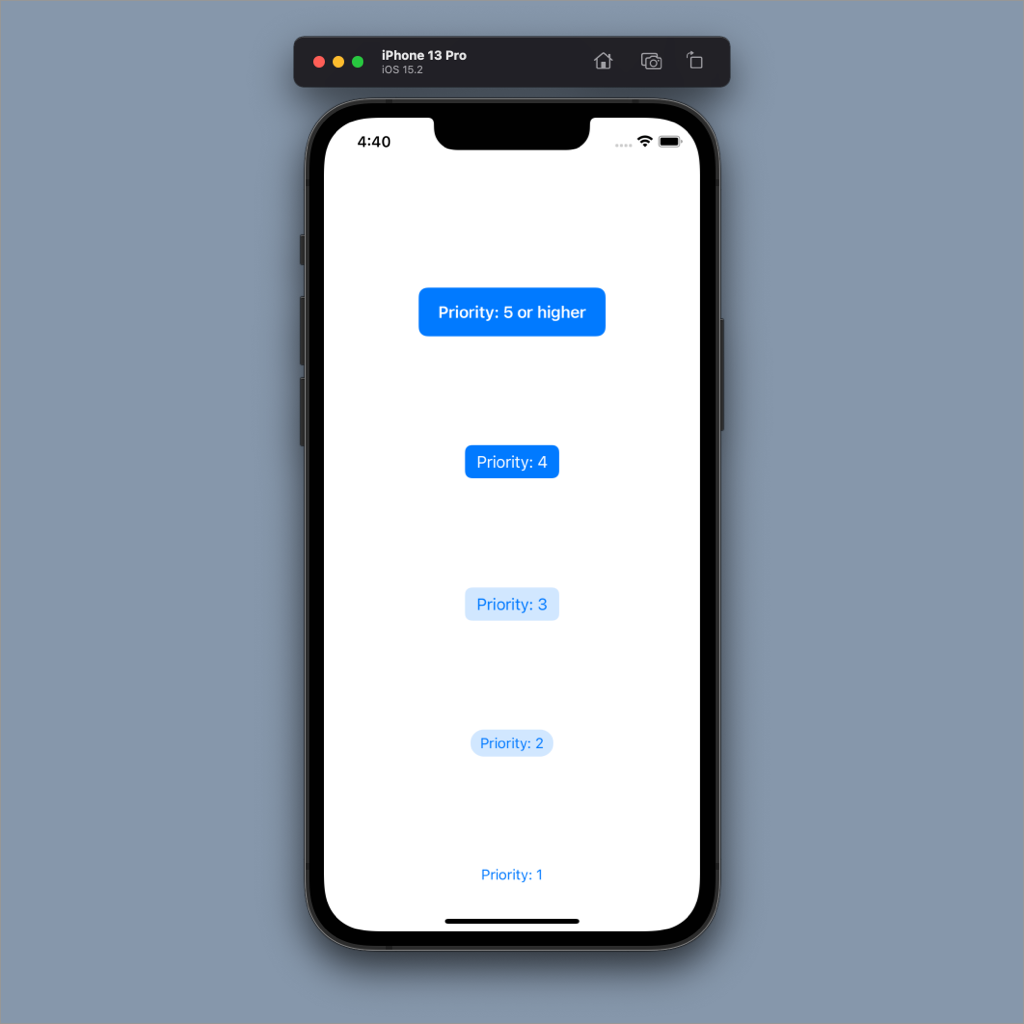
\includegraphics[width=100mm]{img/Button_priority.png}
    \end{center}
    \caption{Buttonの優先度による視覚的目立たせ具合}
    \label{fig:button_priority}
  \end{minipage}
\end{figure}

\subsubsection{Toggle}
図\ref{fig:button_priority}のように実装した.Toggleに関しては優先度で大きさや目立たせ具合が変わることはなく,優先度は配置のみに利用する.

\begin{figure}[htbp]
  \begin{minipage}{\hsize}
    \begin{center}
       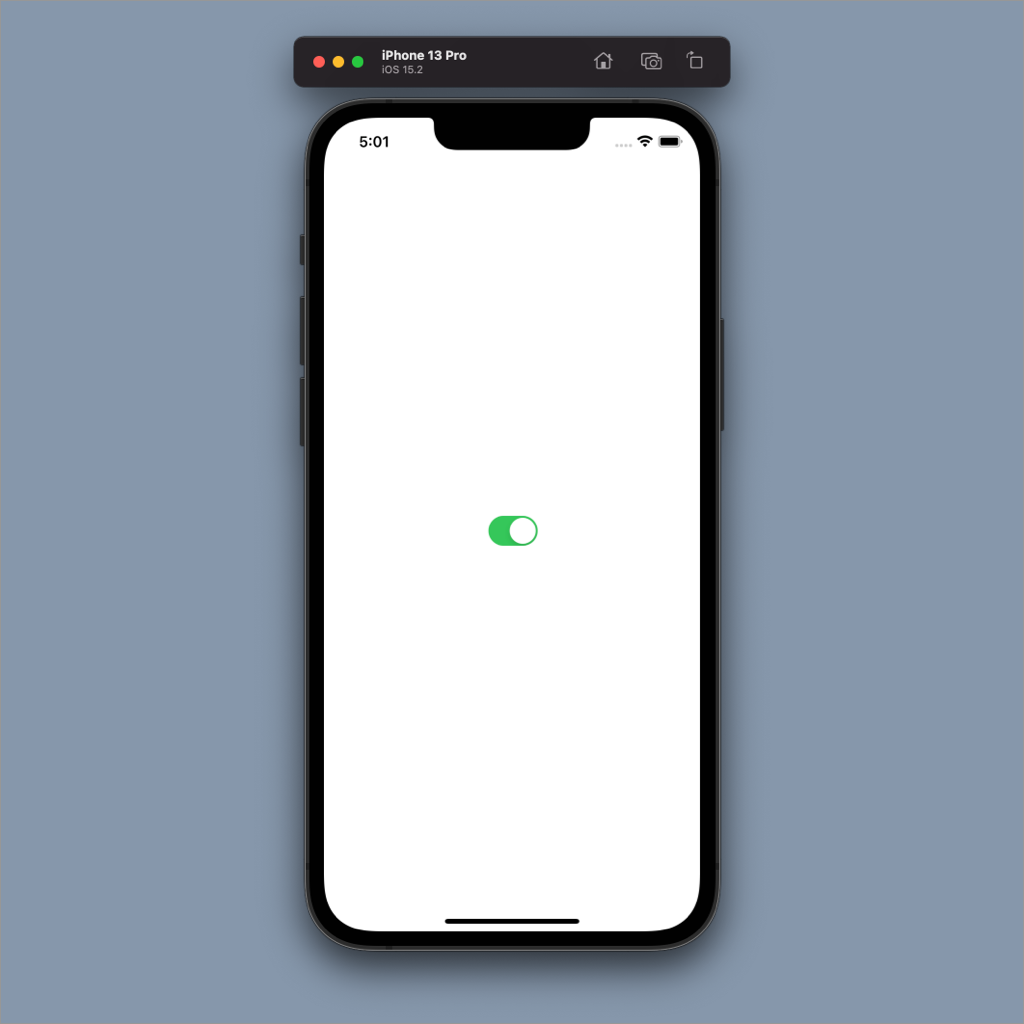
\includegraphics[width=100mm]{img/Toggle_priority.png}
    \end{center}
    \caption{Toggleの優先度による視覚的目立たせ具合}
    \label{fig:toggle_priority}
  \end{minipage}
\end{figure}

\subsubsection{Image}
図\ref{fig:image_priority}のように実装した.Imageは優先度/ 10の高さを持つ.表\ref{fig:image_priority}で使用しているサンプル画像が切れずに全てが映るようにしているため.6以上でも大きさが変化していない.

\begin{figure}[htbp]
  \begin{minipage}{\hsize}
    \begin{center}
       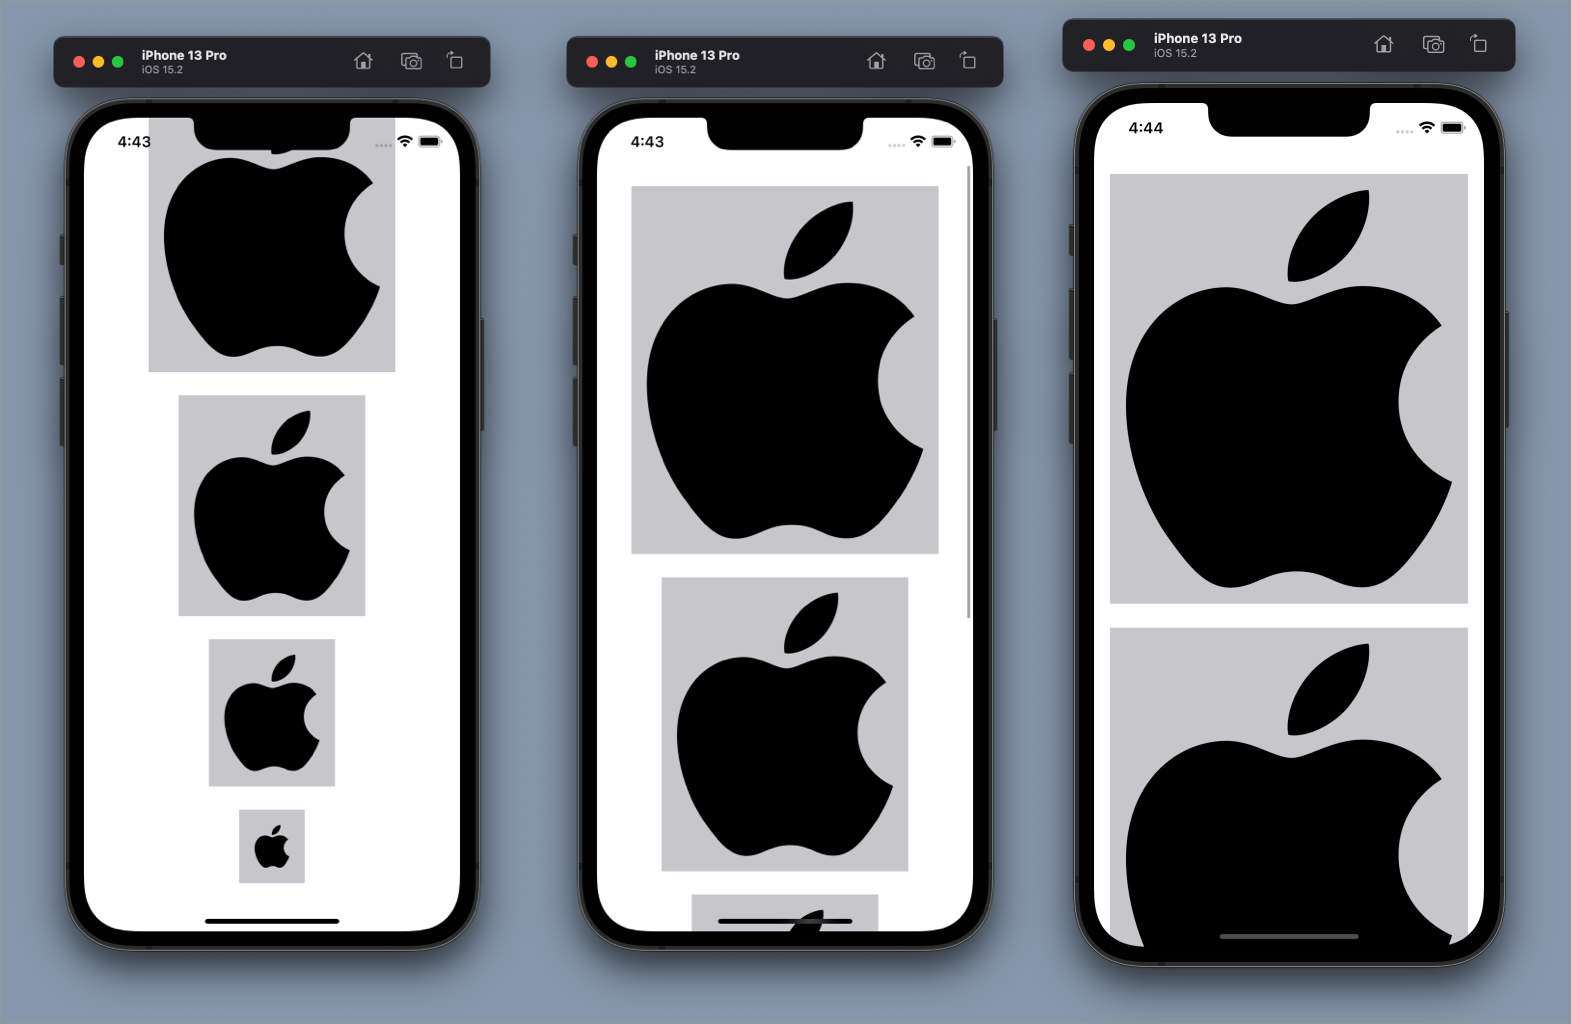
\includegraphics[width=100mm]{img/Image_priority.png}
    \end{center}
    \caption{Imageの優先度による視覚的目立たせ具合}
    \label{fig:image_priority}
  \end{minipage}
\end{figure}

\subsubsection{Map}
図\ref{fig:map_priority}のように実装した.本要素も優先度は配置のみに利用し,目立たせ具合は変化させない.また,本要素はユーザの操作を受け付けるが,特例として画面下に持ってはいかない.
\begin{figure}[htbp]
  \begin{minipage}{\hsize}
    \begin{center}
       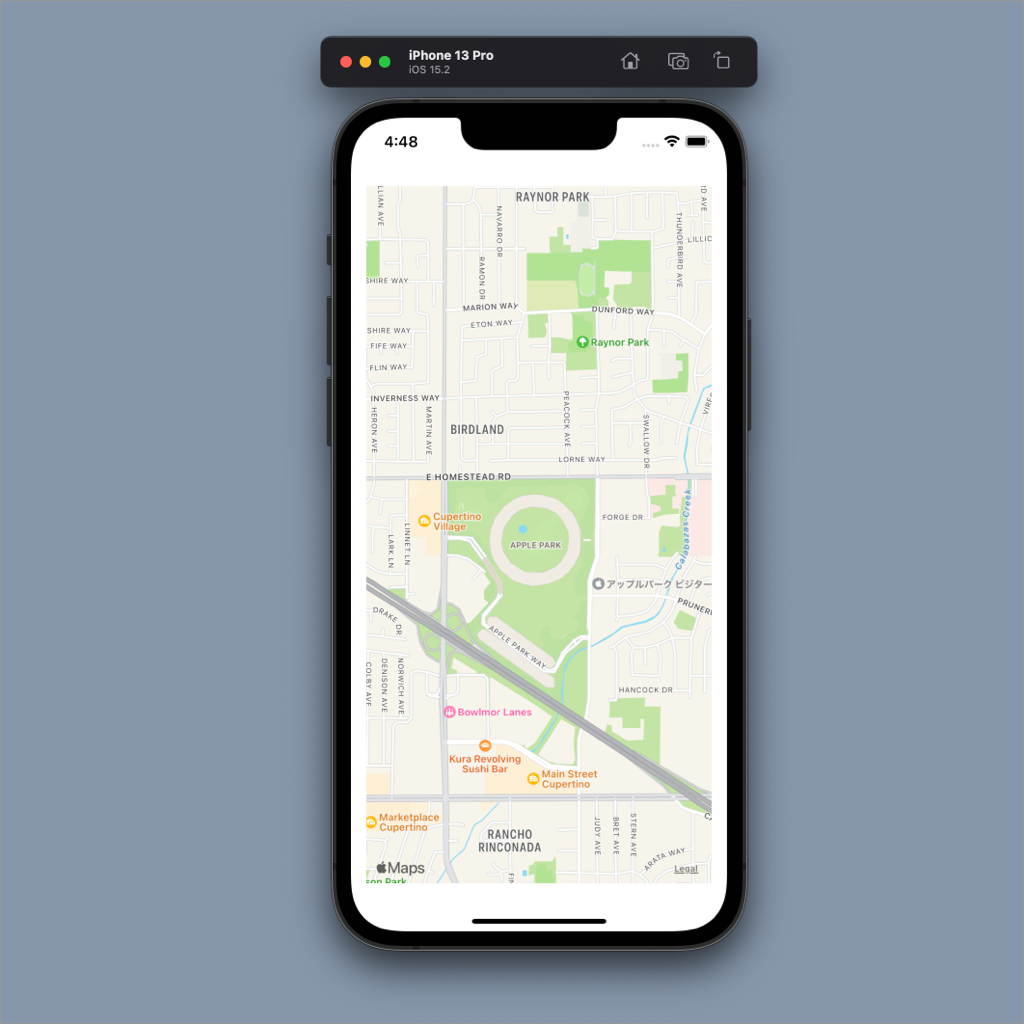
\includegraphics[width=100mm]{img/Map_priority.png}
    \end{center}
    \caption{Mapの優先度による視覚的目立たせ具合}
    \label{fig:map_priority}
  \end{minipage}
\end{figure}

\subsubsection{DatePicker}
図\ref{fig:datepicker_priority}のように実装した.優先度1,2では画面右下のコンパクトスタイル,優先度3ではドラムロールスタイル,4以上ではカレンダースタイルで日付を選ぶようにした.でもこれ以上の大きさになることはなく,余白として扱われる.

\begin{figure}[htbp]
  \begin{minipage}{\hsize}
    \begin{center}
       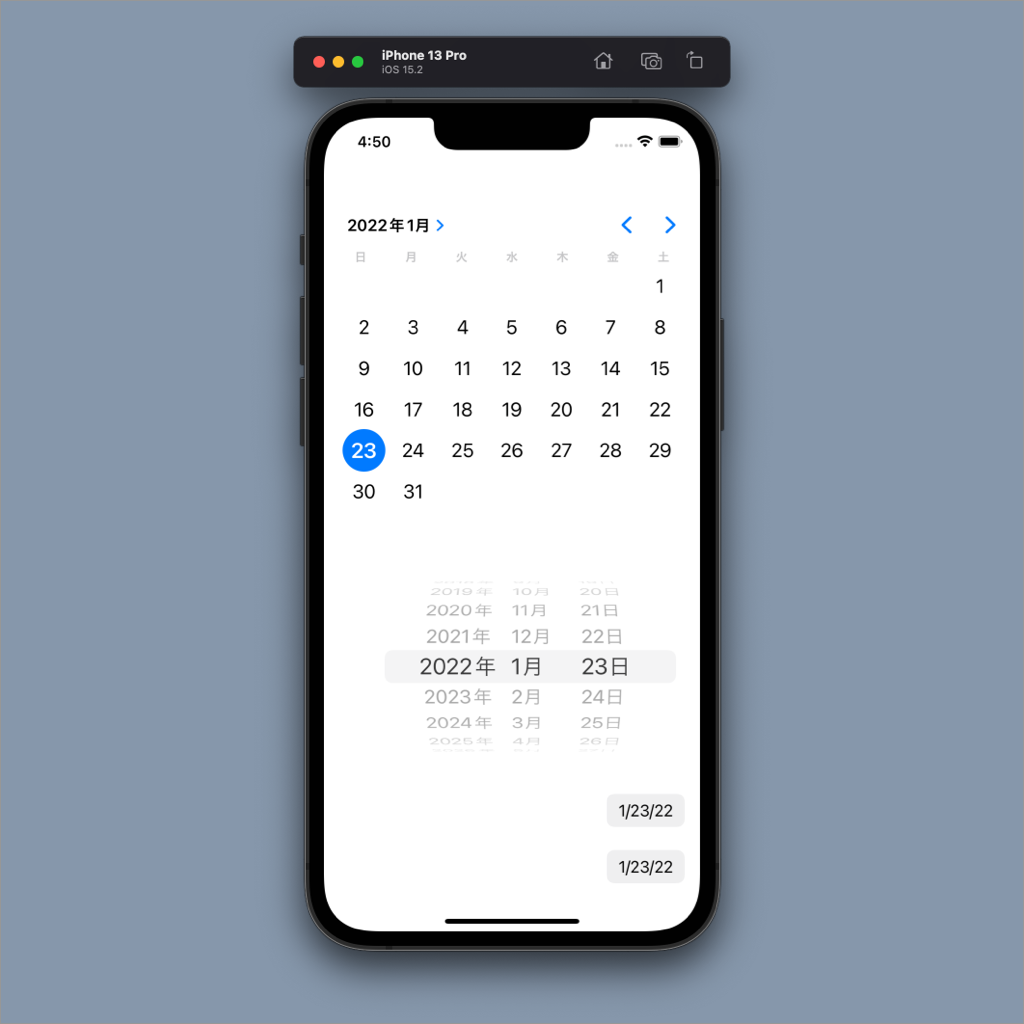
\includegraphics[width=100mm]{img/DatePicker_priority.png}
    \end{center}
    \caption{DatePickerの優先度による視覚的目立たせ具合}
    \label{fig:datepicker_priority}
  \end{minipage}
\end{figure}

\subsubsection{Slider}
図\ref{fig:slider_priority}のように実装した.優先度による見た目の変化はなく,配置のみに利用される.

\begin{figure}[htbp]
  \begin{minipage}{\hsize}
    \begin{center}
       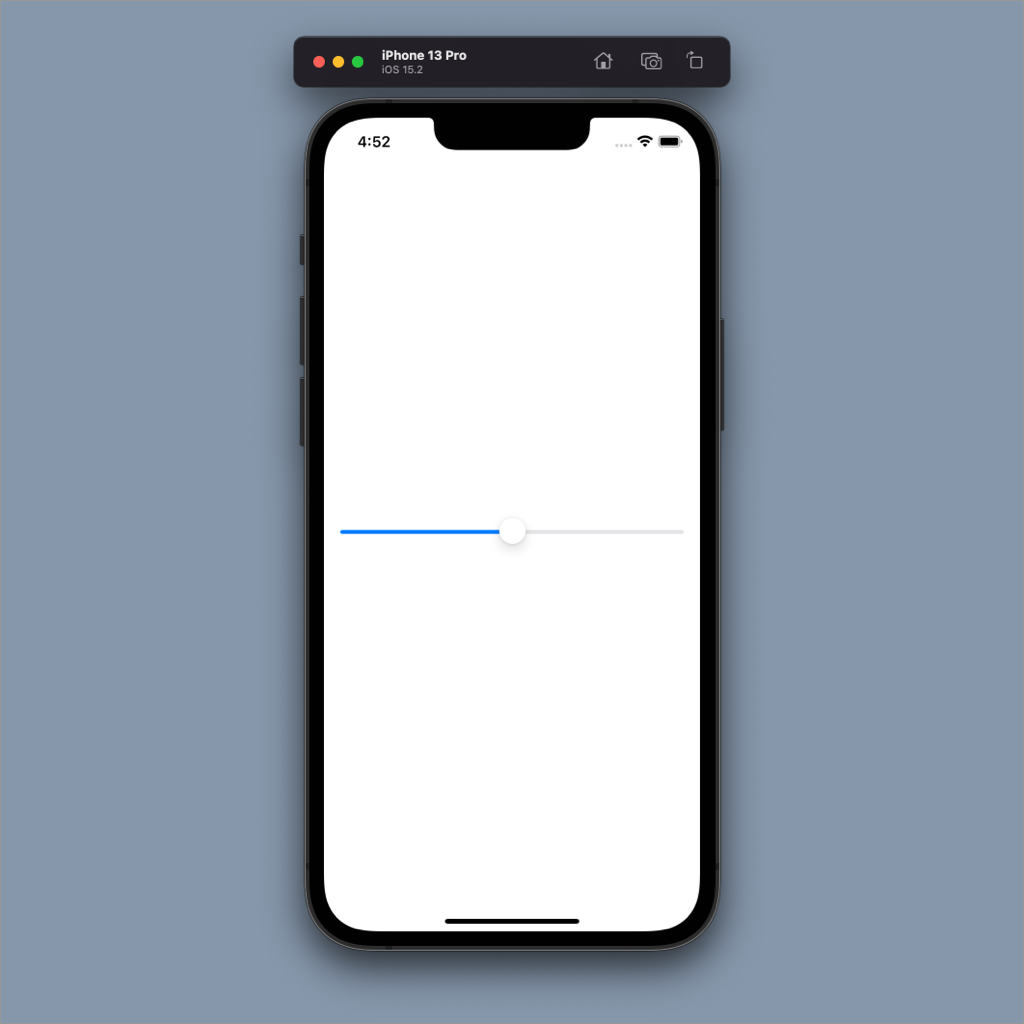
\includegraphics[width=100mm]{img/Slider_priority.png}
    \end{center}
    \caption{Sliderの優先度による視覚的目立たせ具合}
    \label{fig:slider_priority}
  \end{minipage}
\end{figure}


\subsection{グルーピング}
グルーピングでは
\subsubsection{グルーピングの入れ子構造}

\subsection{表示レイアウトアルゴリズム}

\section{システムの有効性についての実験}

\subsection{既存UIの再現}
前セクションでは本システムの表示アルゴリズムの具体的なシステムの実装を説明した.本セクションでは既存UIを要素,優先度,グルーピングに落とし込み,本システムを利用して再度UI構築を行う実験をおこなった.
本実験ではSNSフィード画面(Instagram), ログイン画面(NIKKEI Wave),リスト画面(設定),地図画面(Maps)についておこなった.
\subsubsection{SNSフィード画面(Instagram)}
図\ref{fig:instagram_screenshot}を解析し, 図\ref{fig:instagram_ViewStructure}の要素,優先度グルーピングを得ることができた.図\ref{fig:instagram_ViewStructure}の構造を複数個本システムにインプットしたところ図\ref{fig:instagram_autogen}を得ることができた.


\begin{figure}[htbp]
  \begin{minipage}{\hsize}
    \begin{center}
       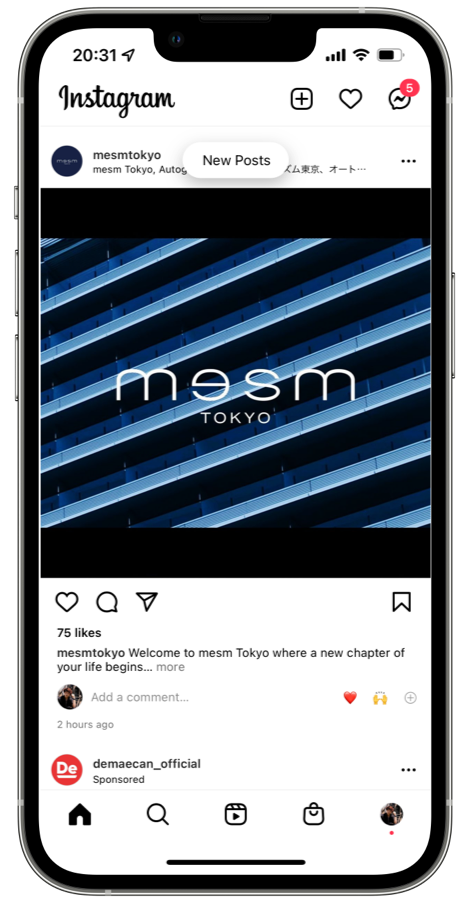
\includegraphics[width=50mm]{img/instagram_screenshot.png}
    \end{center}
    \caption{既存のSNSフィード画面(Instagram)}
    \label{fig:instagram_screenshot}
  \end{minipage}
\end{figure}

\begin{figure}[htbp]
  \begin{minipage}{\hsize}
    \begin{center}
       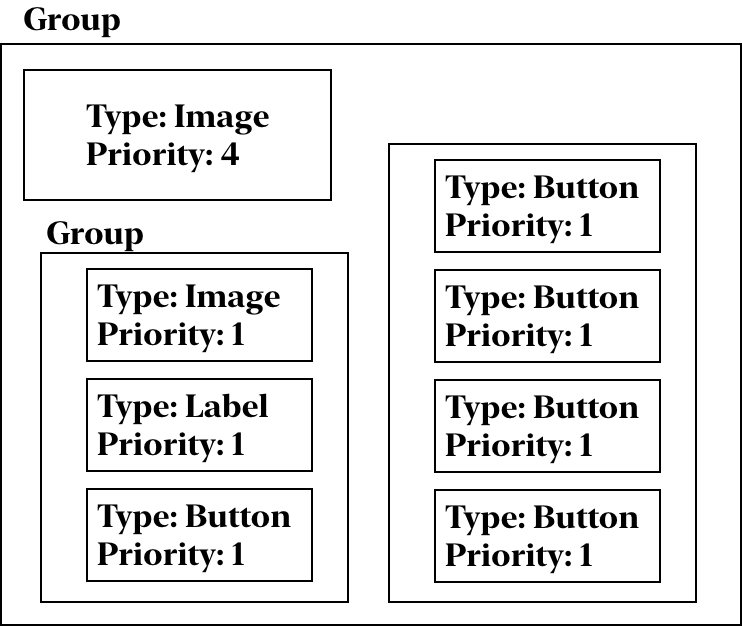
\includegraphics[width=100mm]{img/Instagram_ViewStructure.png}
    \end{center}
    \caption{既存のSNSフィード画面(Instagram)の要素,優先度,グルーピング}
    \label{fig:instagram_ViewStructure}
  \end{minipage}
\end{figure}

\begin{figure}[htbp]
  \begin{minipage}{\hsize}
    \begin{center}
       \includegraphics[width=50mm]{img/Instagram_autogen.png}
    \end{center}
    \caption{本システムで再構築されたSNSフィード画面}
    \label{fig:instagram_autogen}
  \end{minipage}
\end{figure}

\subsubsection{ログイン画面(NIKKEI Wave)}
図\ref{fig:wave_screenshot}を解析し, 図\ref{fig:wave_ViewStructure}の要素,優先度グルーピングを得ることができた.図\ref{fig:wave_ViewStructure}の構造を複数個本システムにインプットしたところ図\ref{fig:wave_autogen}を得ることができた.

\begin{figure}[htbp]
  \begin{minipage}{\hsize}
    \begin{center}
       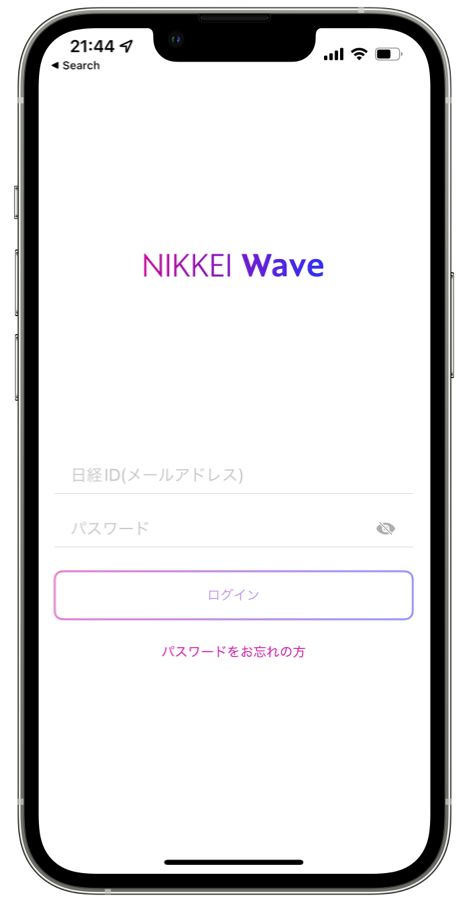
\includegraphics[width=50mm]{img/wave_screenshot.png}
    \end{center}
    \caption{既存のログイン画面(NIKKEI Wave)}
    \label{fig:wave_screenshot}
  \end{minipage}
\end{figure}

\begin{figure}[htbp]
  \begin{minipage}{\hsize}
    \begin{center}
       \includegraphics[width=100mm]{img/wave_ViewStructure.png}
    \end{center}
    \caption{既存のログイン画面(NIKKEI Wave)の要素,優先度,グルーピング}
    \label{fig:wave_ViewStructure}
  \end{minipage}
\end{figure}

\begin{figure}[htbp]
  \begin{minipage}{\hsize}
    \begin{center}
       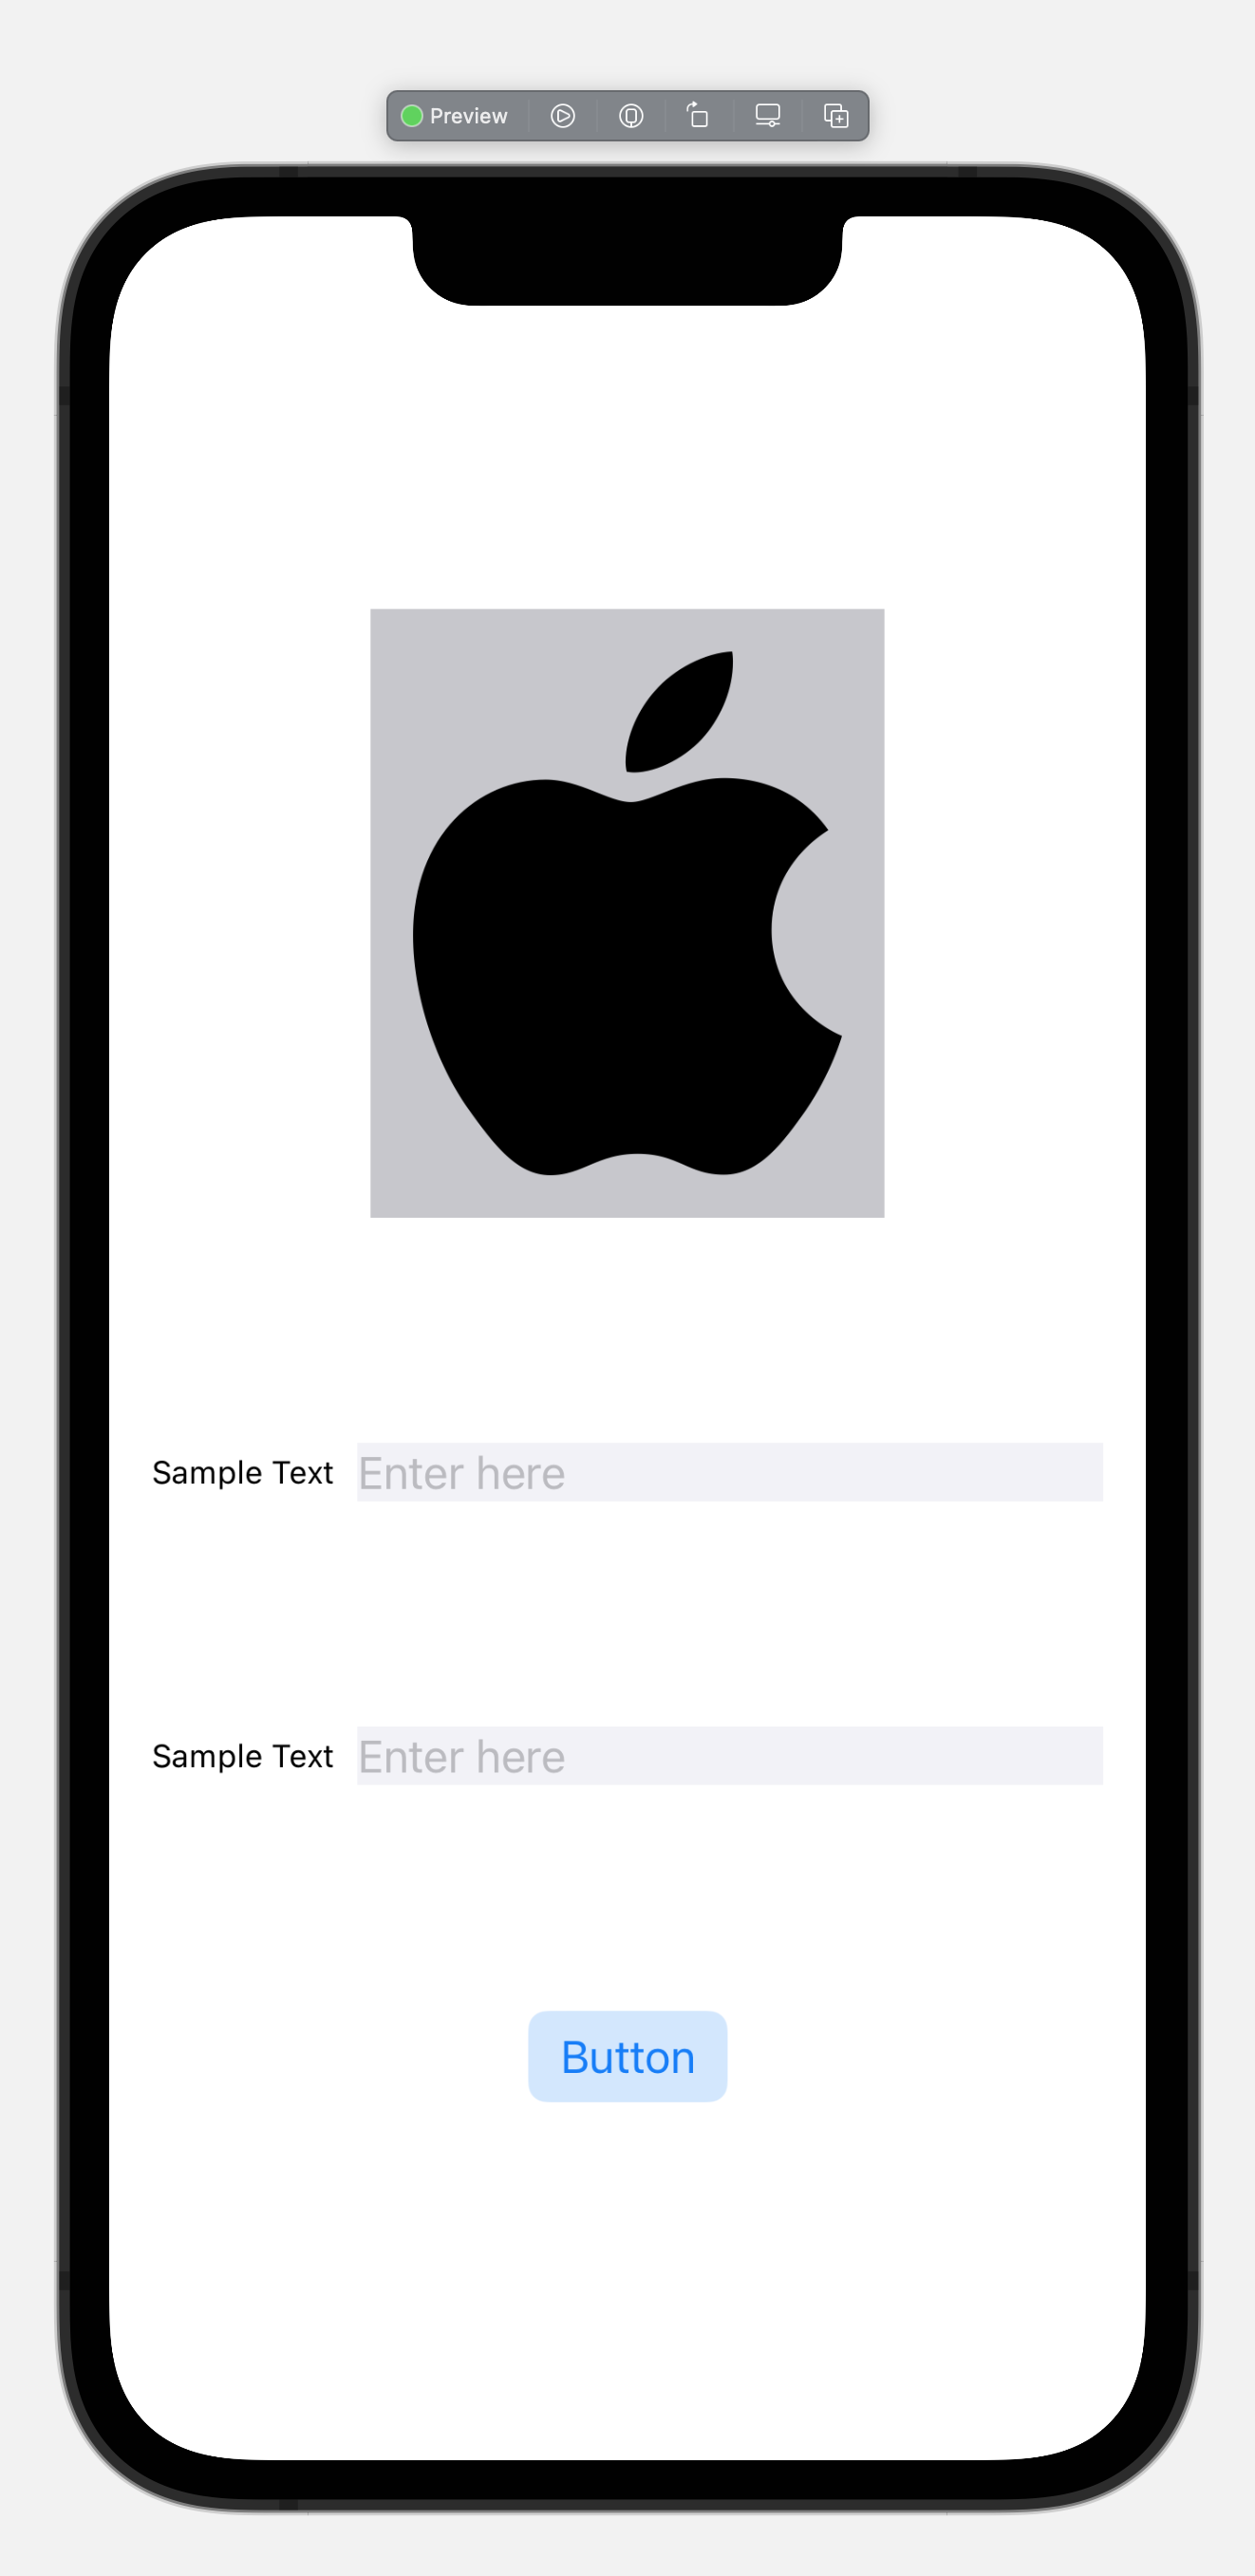
\includegraphics[width=50mm]{img/wave_autogen.png}
    \end{center}
    \caption{本システムで再構築されたログイン画面}
    \label{fig:wave_autogen}
  \end{minipage}
\end{figure}

\subsubsection{リスト画面(設定)}
図\ref{fig:Settings_screenshot}を解析し, 図\ref{fig:Settings_ViewStructure}の要素,優先度グルーピングを得ることができた.図\ref{fig:Settings_ViewStructure}の構造を複数個本システムにインプットしたところ図\ref{fig:Settings_autogen}を得ることができた.

\begin{figure}[htbp]
  \begin{minipage}{\hsize}
    \begin{center}
       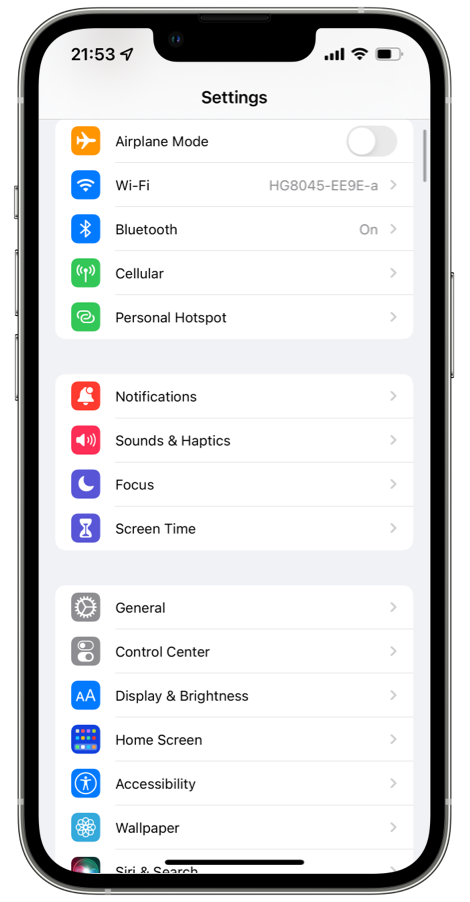
\includegraphics[width=50mm]{img/Settings_screenshot.png}
    \end{center}
    \caption{リスト画面(Settings)}
    \label{fig:Settings_screenshot}
  \end{minipage}
\end{figure}

\begin{figure}[htbp]
  \begin{minipage}{\hsize}
    \begin{center}
       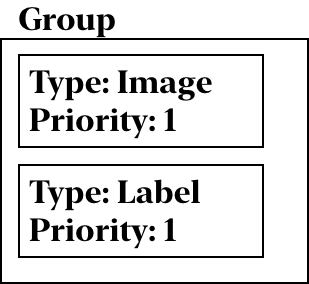
\includegraphics[width=30mm]{img/Settings_ViewStructure.png}
    \end{center}
    \caption{リスト画面(Settings)の要素,優先度,グルーピング}
    \label{fig:Settings_ViewStructure}
  \end{minipage}
\end{figure}

\begin{figure}[htbp]
  \begin{minipage}{\hsize}
    \begin{center}
       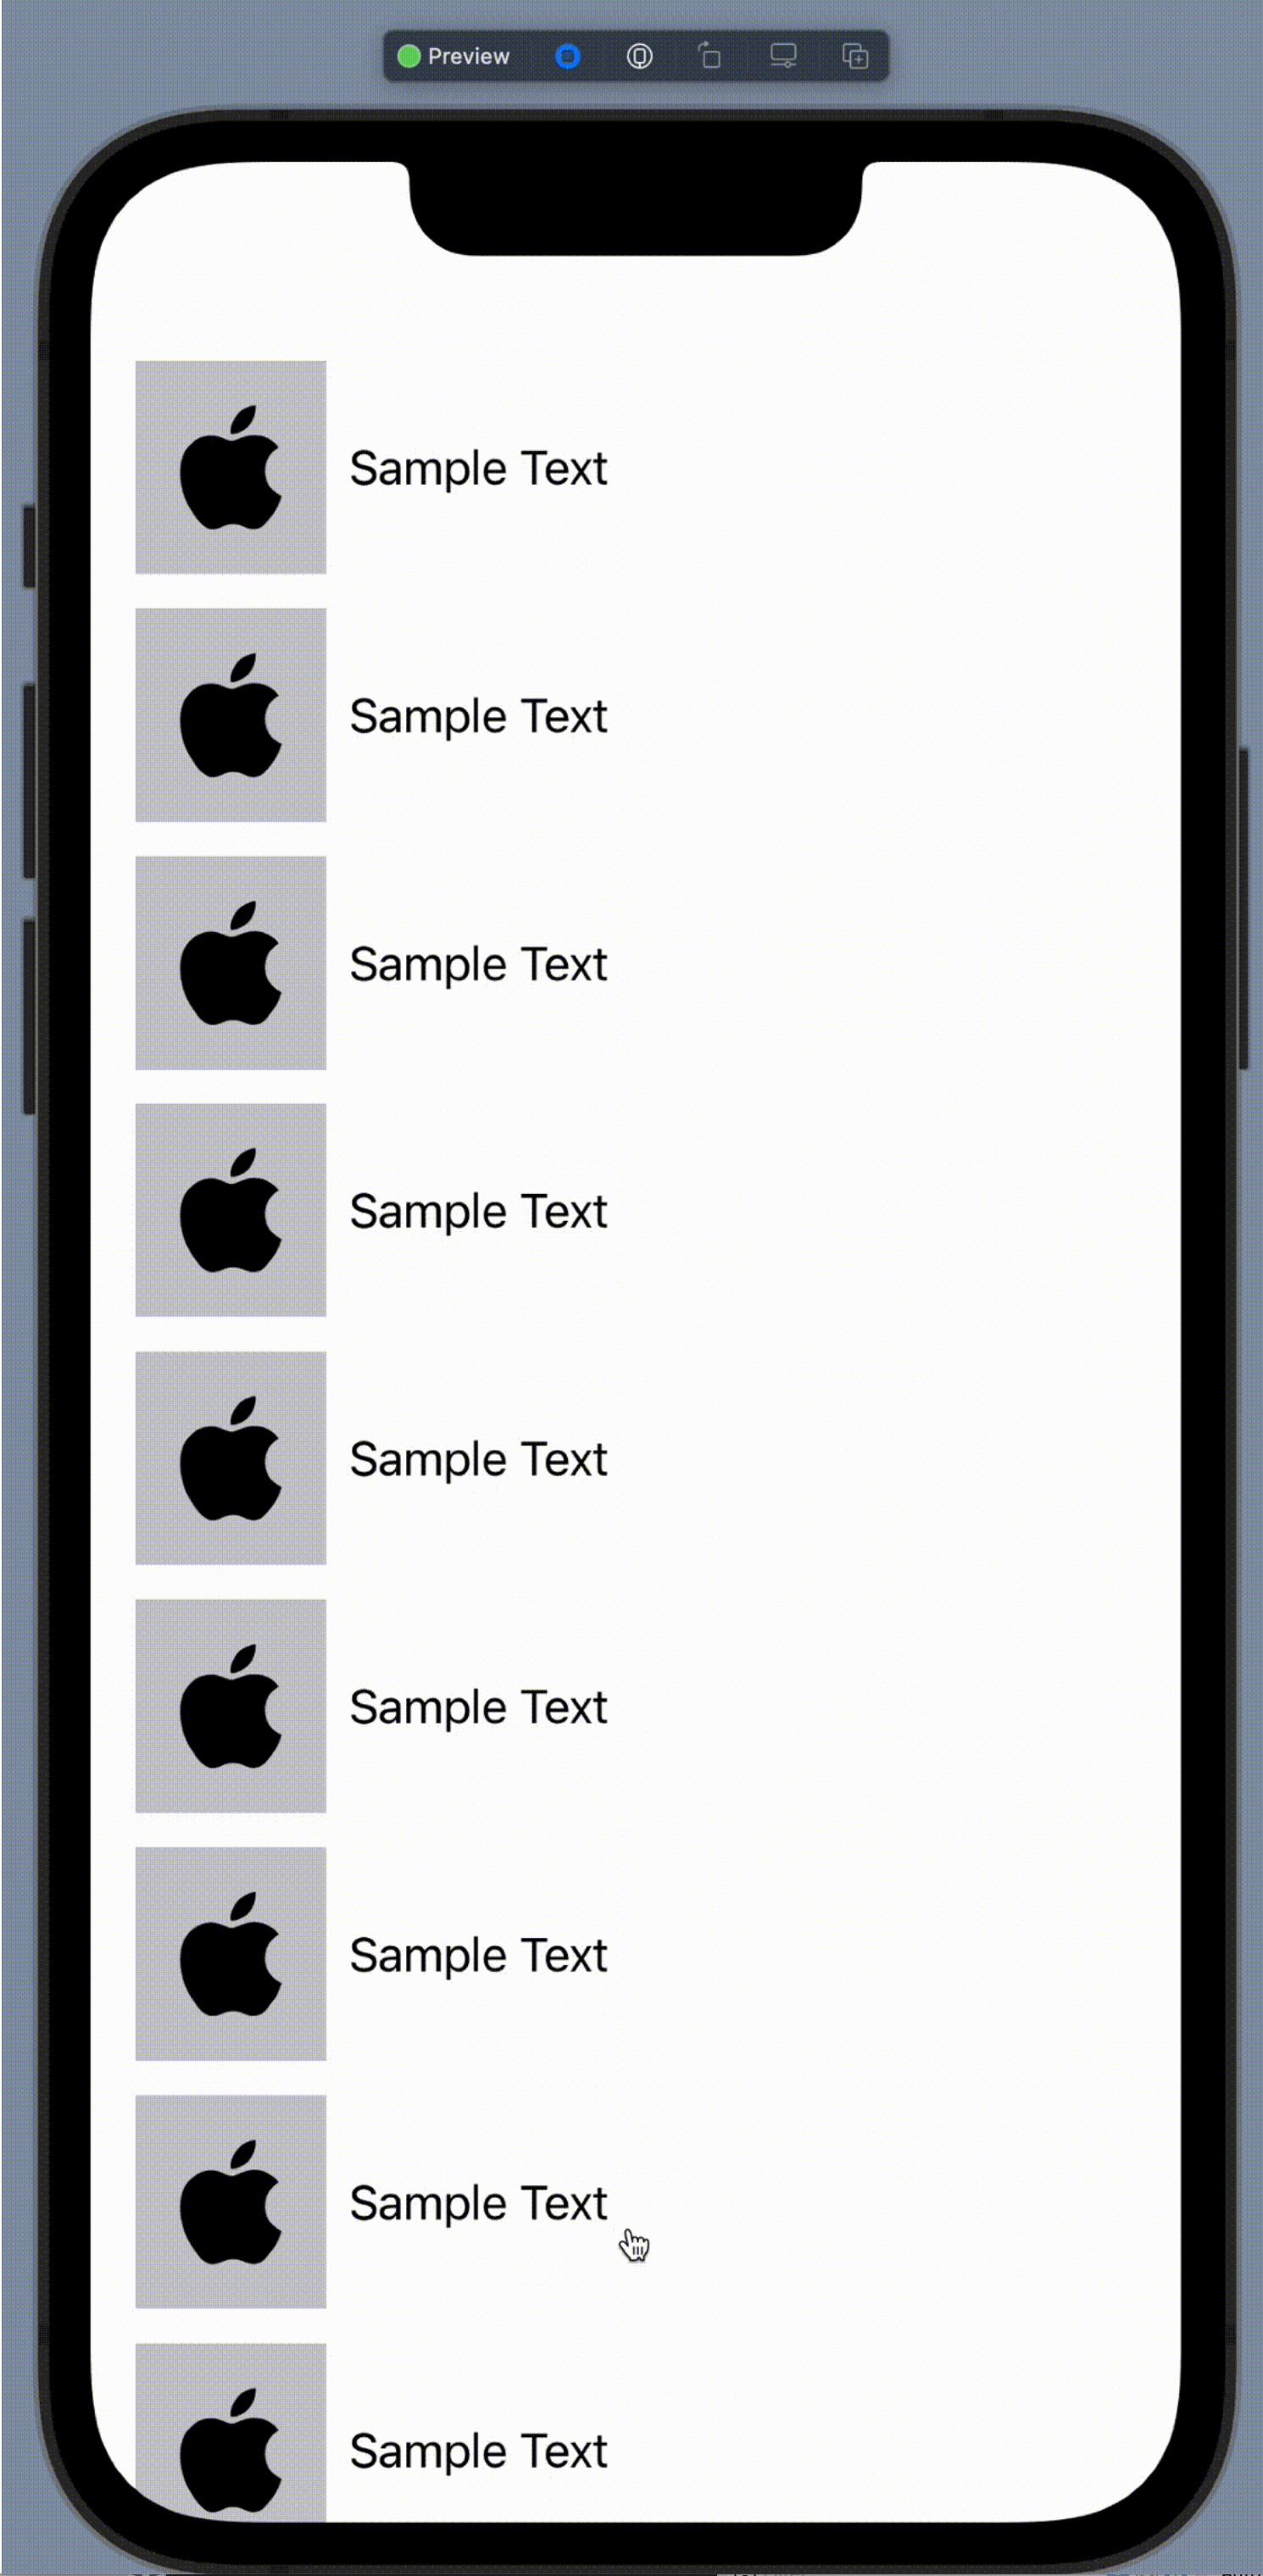
\includegraphics[width=50mm]{img/Settings_autogen.png}
    \end{center}
    \caption{リスト画面}
    \label{fig:Settings_autogen}
  \end{minipage}
\end{figure}


\subsubsection{地図画面(Maps)}
図\ref{fig:Maps_screenshot}を解析し, 図\ref{fig:Maps_ViewStructure}の要素,優先度グルーピングを得ることができた.図\ref{fig:Maps_ViewStructure}の構造を複数個本システムにインプットしたところ図\ref{fig:Maps_autogen}を得ることができた.


\begin{figure}[htbp]
  \begin{minipage}{\hsize}
    \begin{center}
       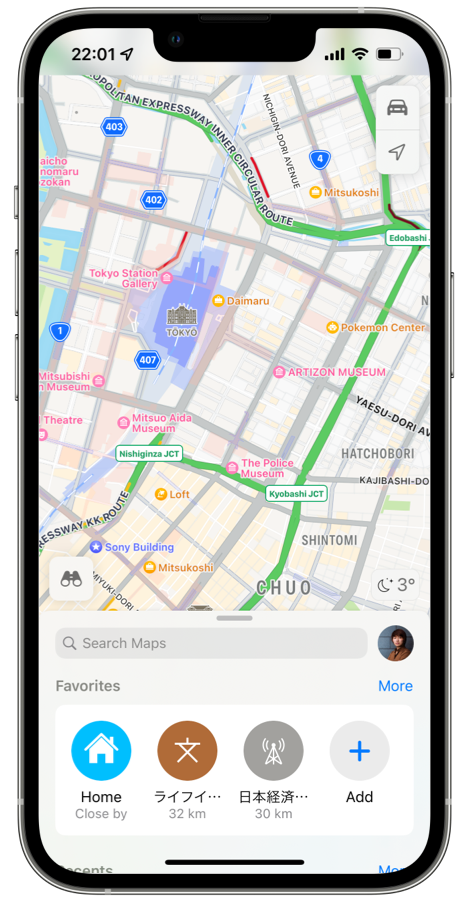
\includegraphics[width=50mm]{img/Maps_screenshot.png}
    \end{center}
    \caption{地図画面(Maps)}
    \label{fig:Maps_screenshot}
  \end{minipage}
\end{figure}

\begin{figure}[htbp]
  \begin{minipage}{\hsize}
    \begin{center}
       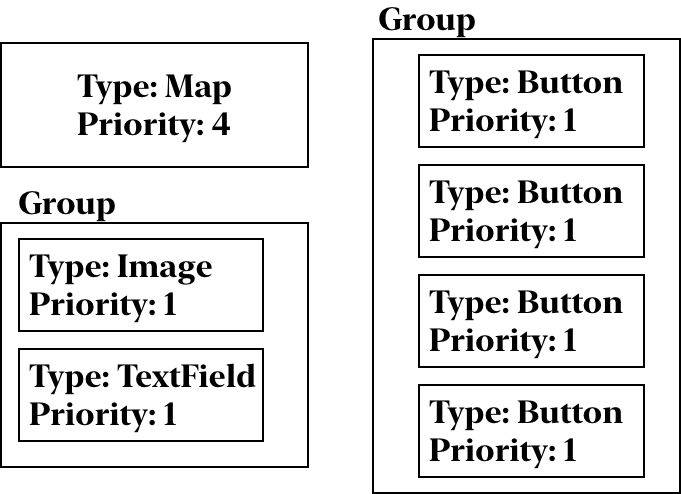
\includegraphics[width=100mm]{img/Maps_ViewStructure.png}
    \end{center}
    \caption{地図画面(Maps)の要素,優先度,グルーピング}
    \label{fig:Maps_ViewStructure}
  \end{minipage}
\end{figure}

\begin{figure}[htbp]
  \begin{minipage}{\hsize}
    \begin{center}
       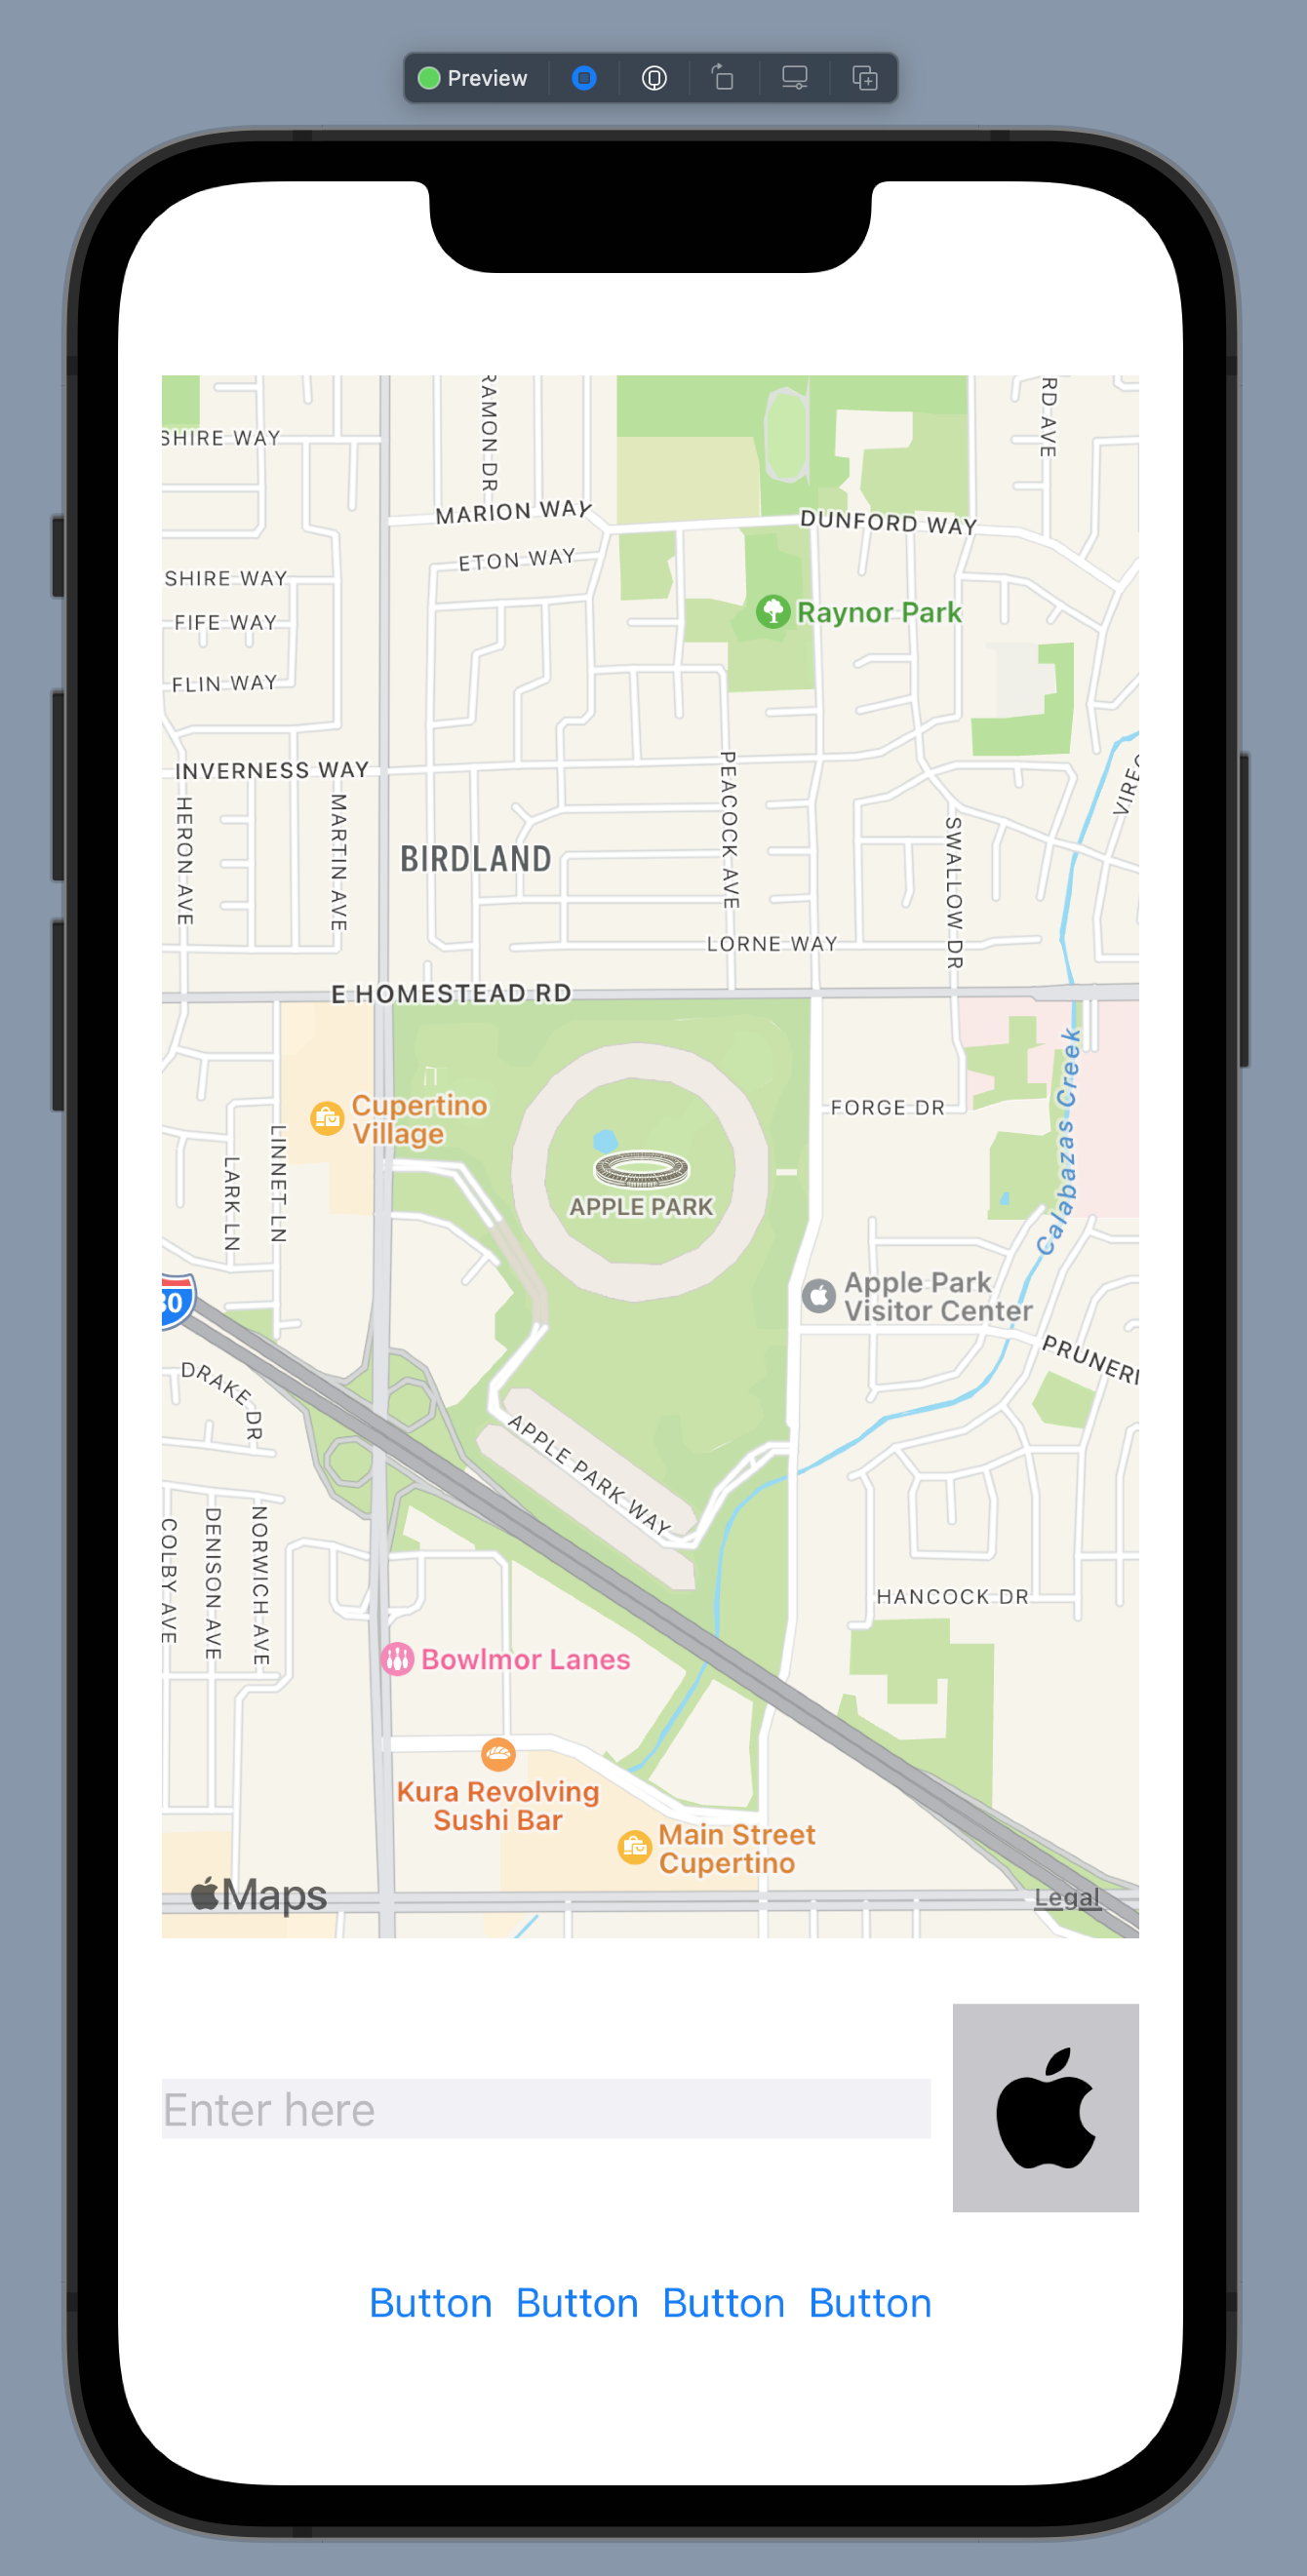
\includegraphics[width=50mm]{img/Maps_autogen.png}
    \end{center}
    \caption{地図画面}
    \label{fig:Maps_autogen}
  \end{minipage}
\end{figure}


\subsection{ユーザテスト}
普段からiOSネイティブアプリケーションの企画,設計,開発を行う14-17歳の中高生男女を対象に設計段階のアプリにおいて本システムを利用しUIの自動生成の有用性を測る実験とアンケートを実施した.
本ユーザテストでは従来のUIデザイン手法ではなく,画面内の要素,優先度,グルーピングを抽出することの難易度調査,期待するUIが自動生成されるかどうか,また優先度を編集することでの本システムとのインタラクションによるUI設計があるかを調査した.
\subsection{対象と手続き}
本ユーザテストではコンピュータの基本操作は理解しており,日頃からiOSネイティブアプリケーションの企画,設計,開発をおこなっている14-17歳の中高生を対象とした.

被験者には事前説明として画面内の要素,優先度,グルーピングで構成できる旨の説明を行い,使用できる要素の種類一覧(表\ref{table:ui_elements})を示した.

実験では白紙一枚を渡し,白紙に図\ref{fig:instagram_ViewStructure},図\ref{fig:wave_ViewStructure},図\ref{fig:Settings_ViewStructure},図\ref{fig:Maps_ViewStructure},にならった 要素,優先度,グルーピングの図示を行わせ,自動生成システムにかけ実際にUIを出力させた.


\begin{figure}[htbp]
  \begin{minipage}{\hsize}
    \begin{center}
       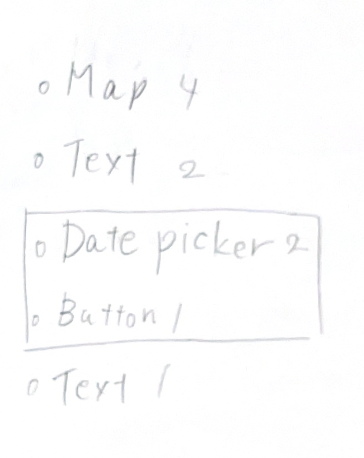
\includegraphics[width=50mm]{img/usertest_viewstructure_1.png}
    \end{center}
    \caption{被験者A記入用紙}
    \label{fig:usertest_viewstructure_1}
  \end{minipage}
\end{figure}

\begin{figure}[htbp]
  \begin{minipage}{\hsize}
    \begin{center}
       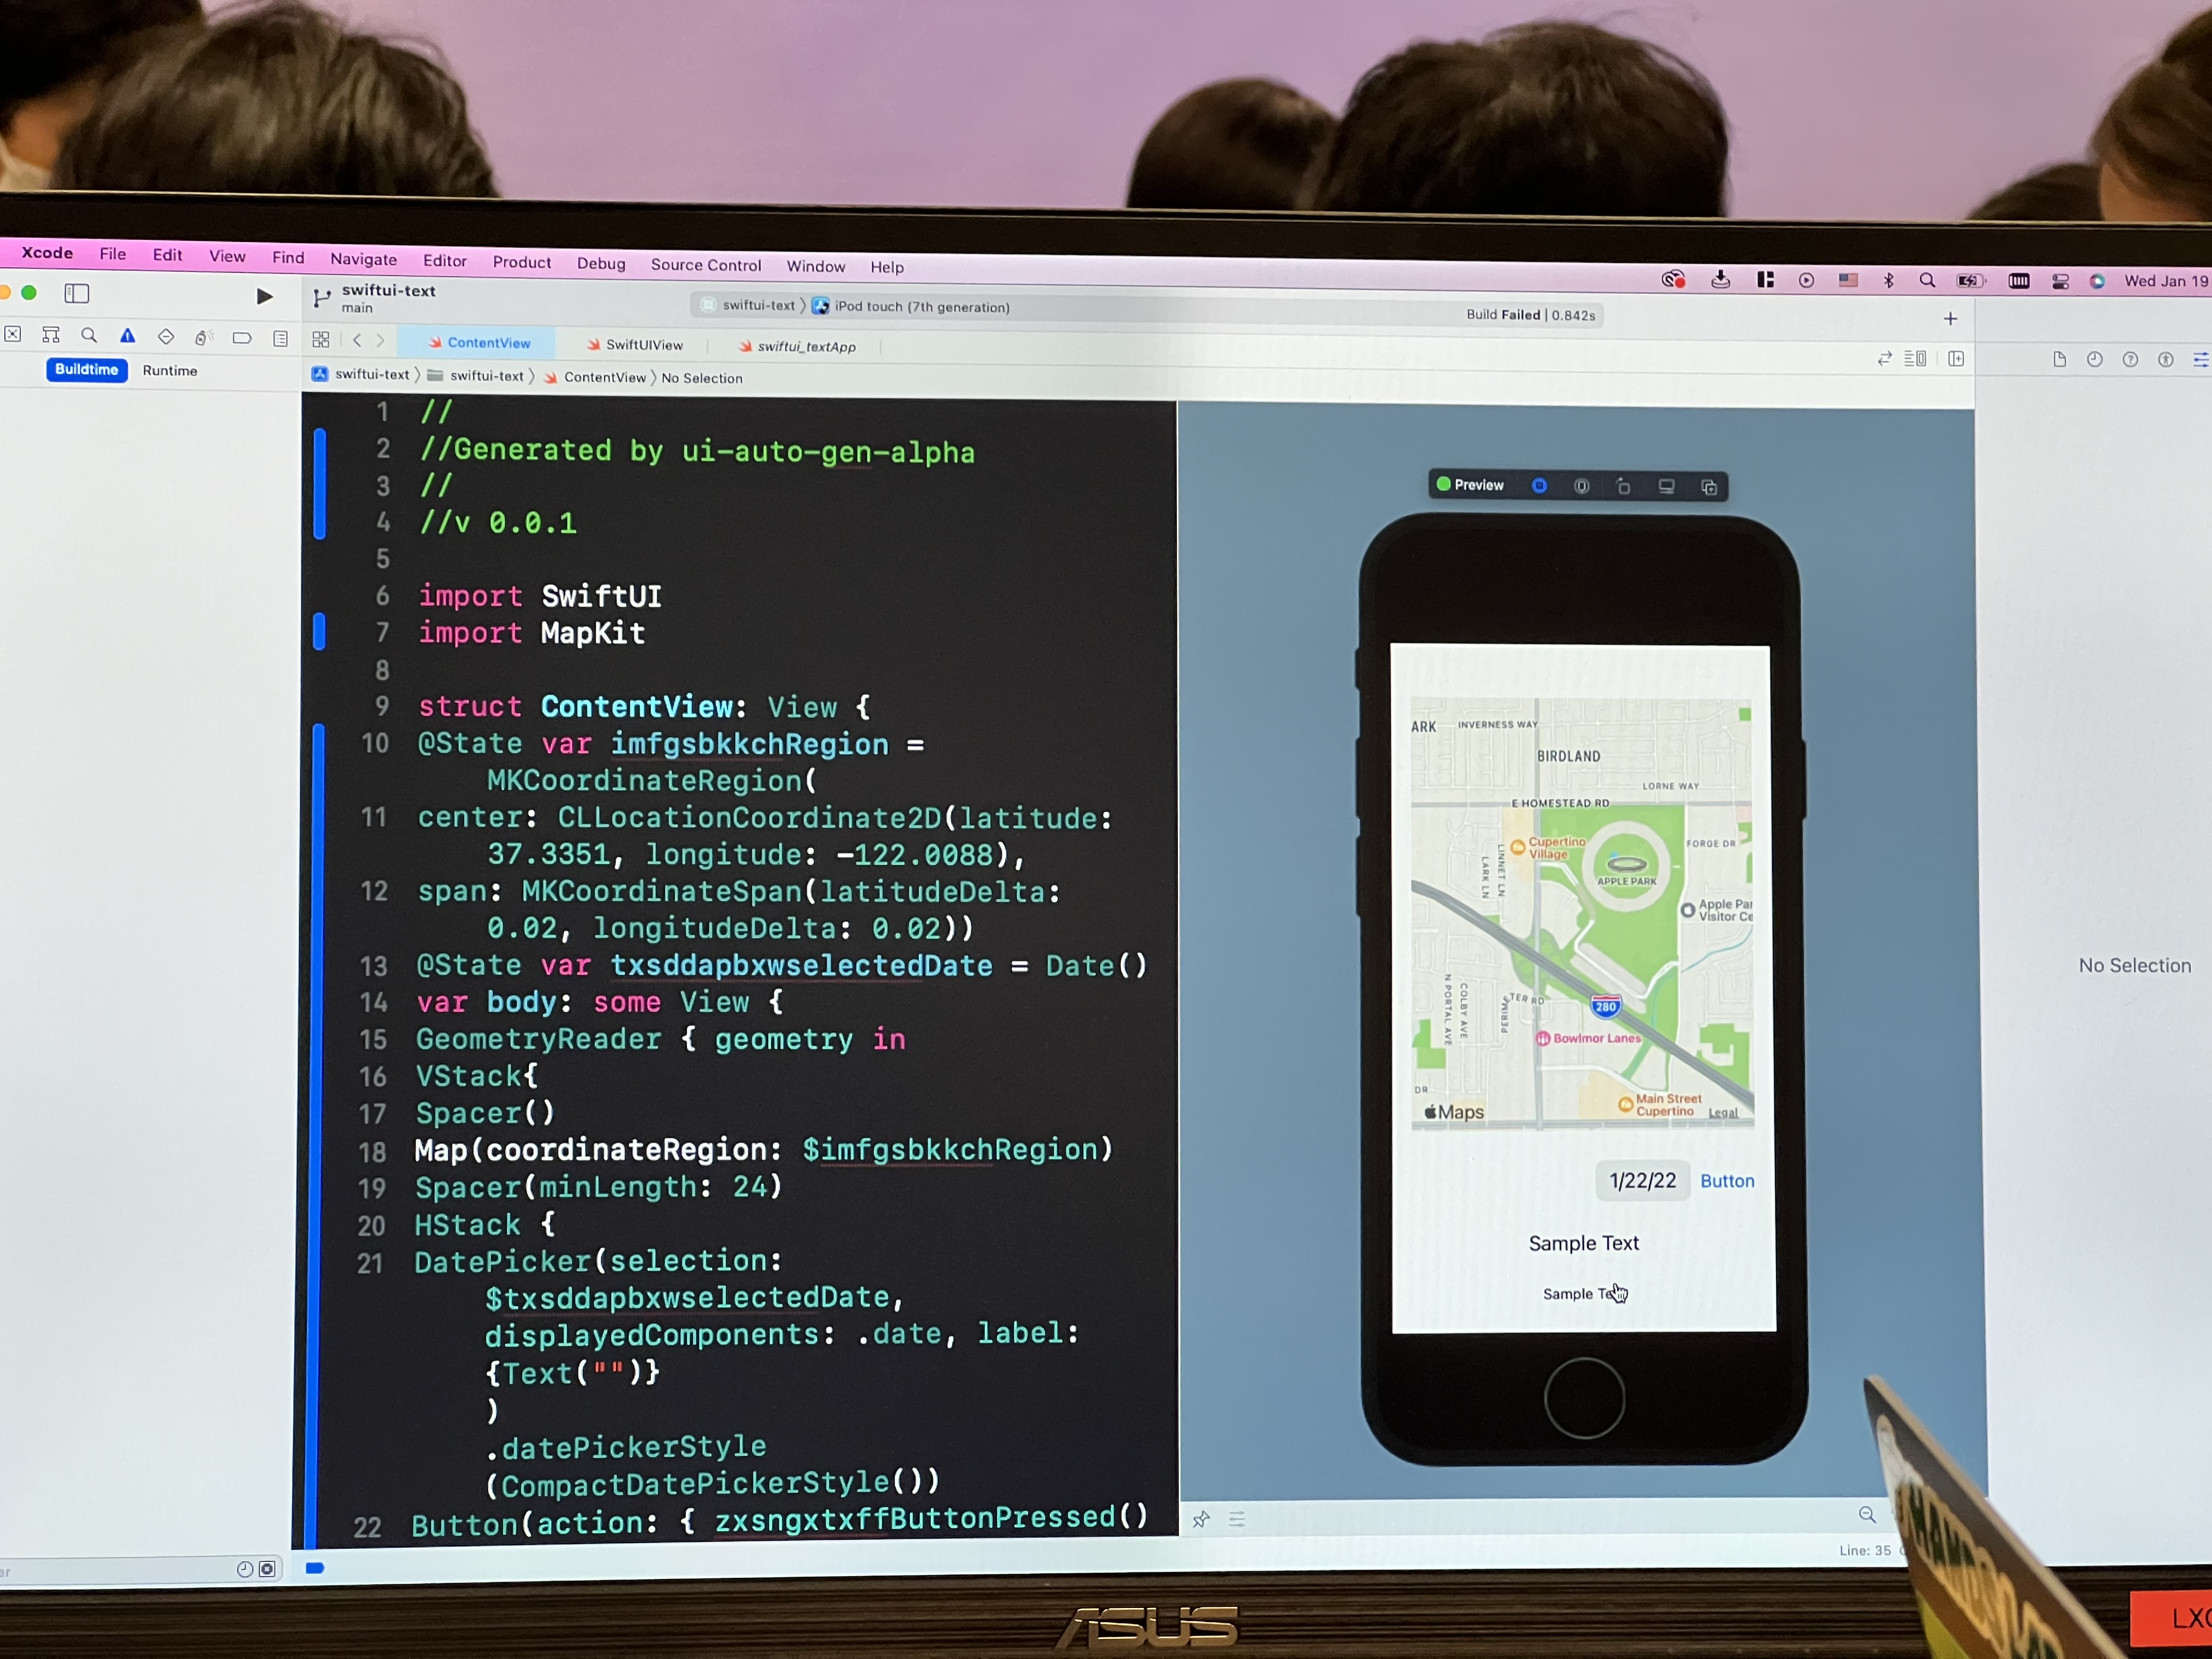
\includegraphics[width=100mm]{img/usertest_autogen_1.jpeg}
    \end{center}
    \caption{被験者A自動生成UI}
    \label{fig:usertest_autogen_1}
  \end{minipage}
\end{figure}



\begin{figure}[htbp]
  \begin{minipage}{\hsize}
    \begin{center}
       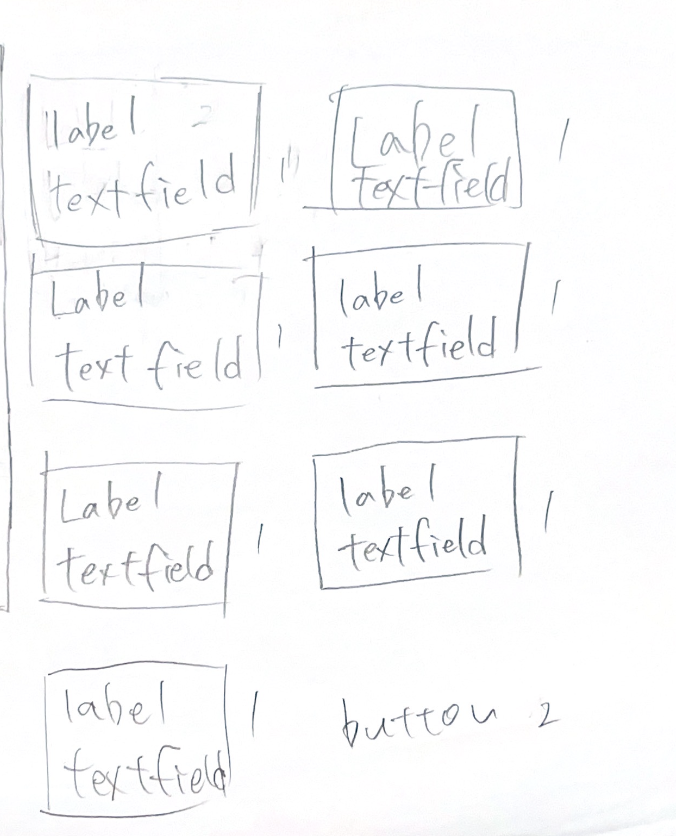
\includegraphics[width=50mm]{img/usertest_viewstructure_2.png}
    \end{center}
    \caption{被験者B記入用紙}
    \label{fig:usertest_viewstructure_2}
  \end{minipage}
\end{figure}

\begin{figure}[htbp]
  \begin{minipage}{\hsize}
    \begin{center}
       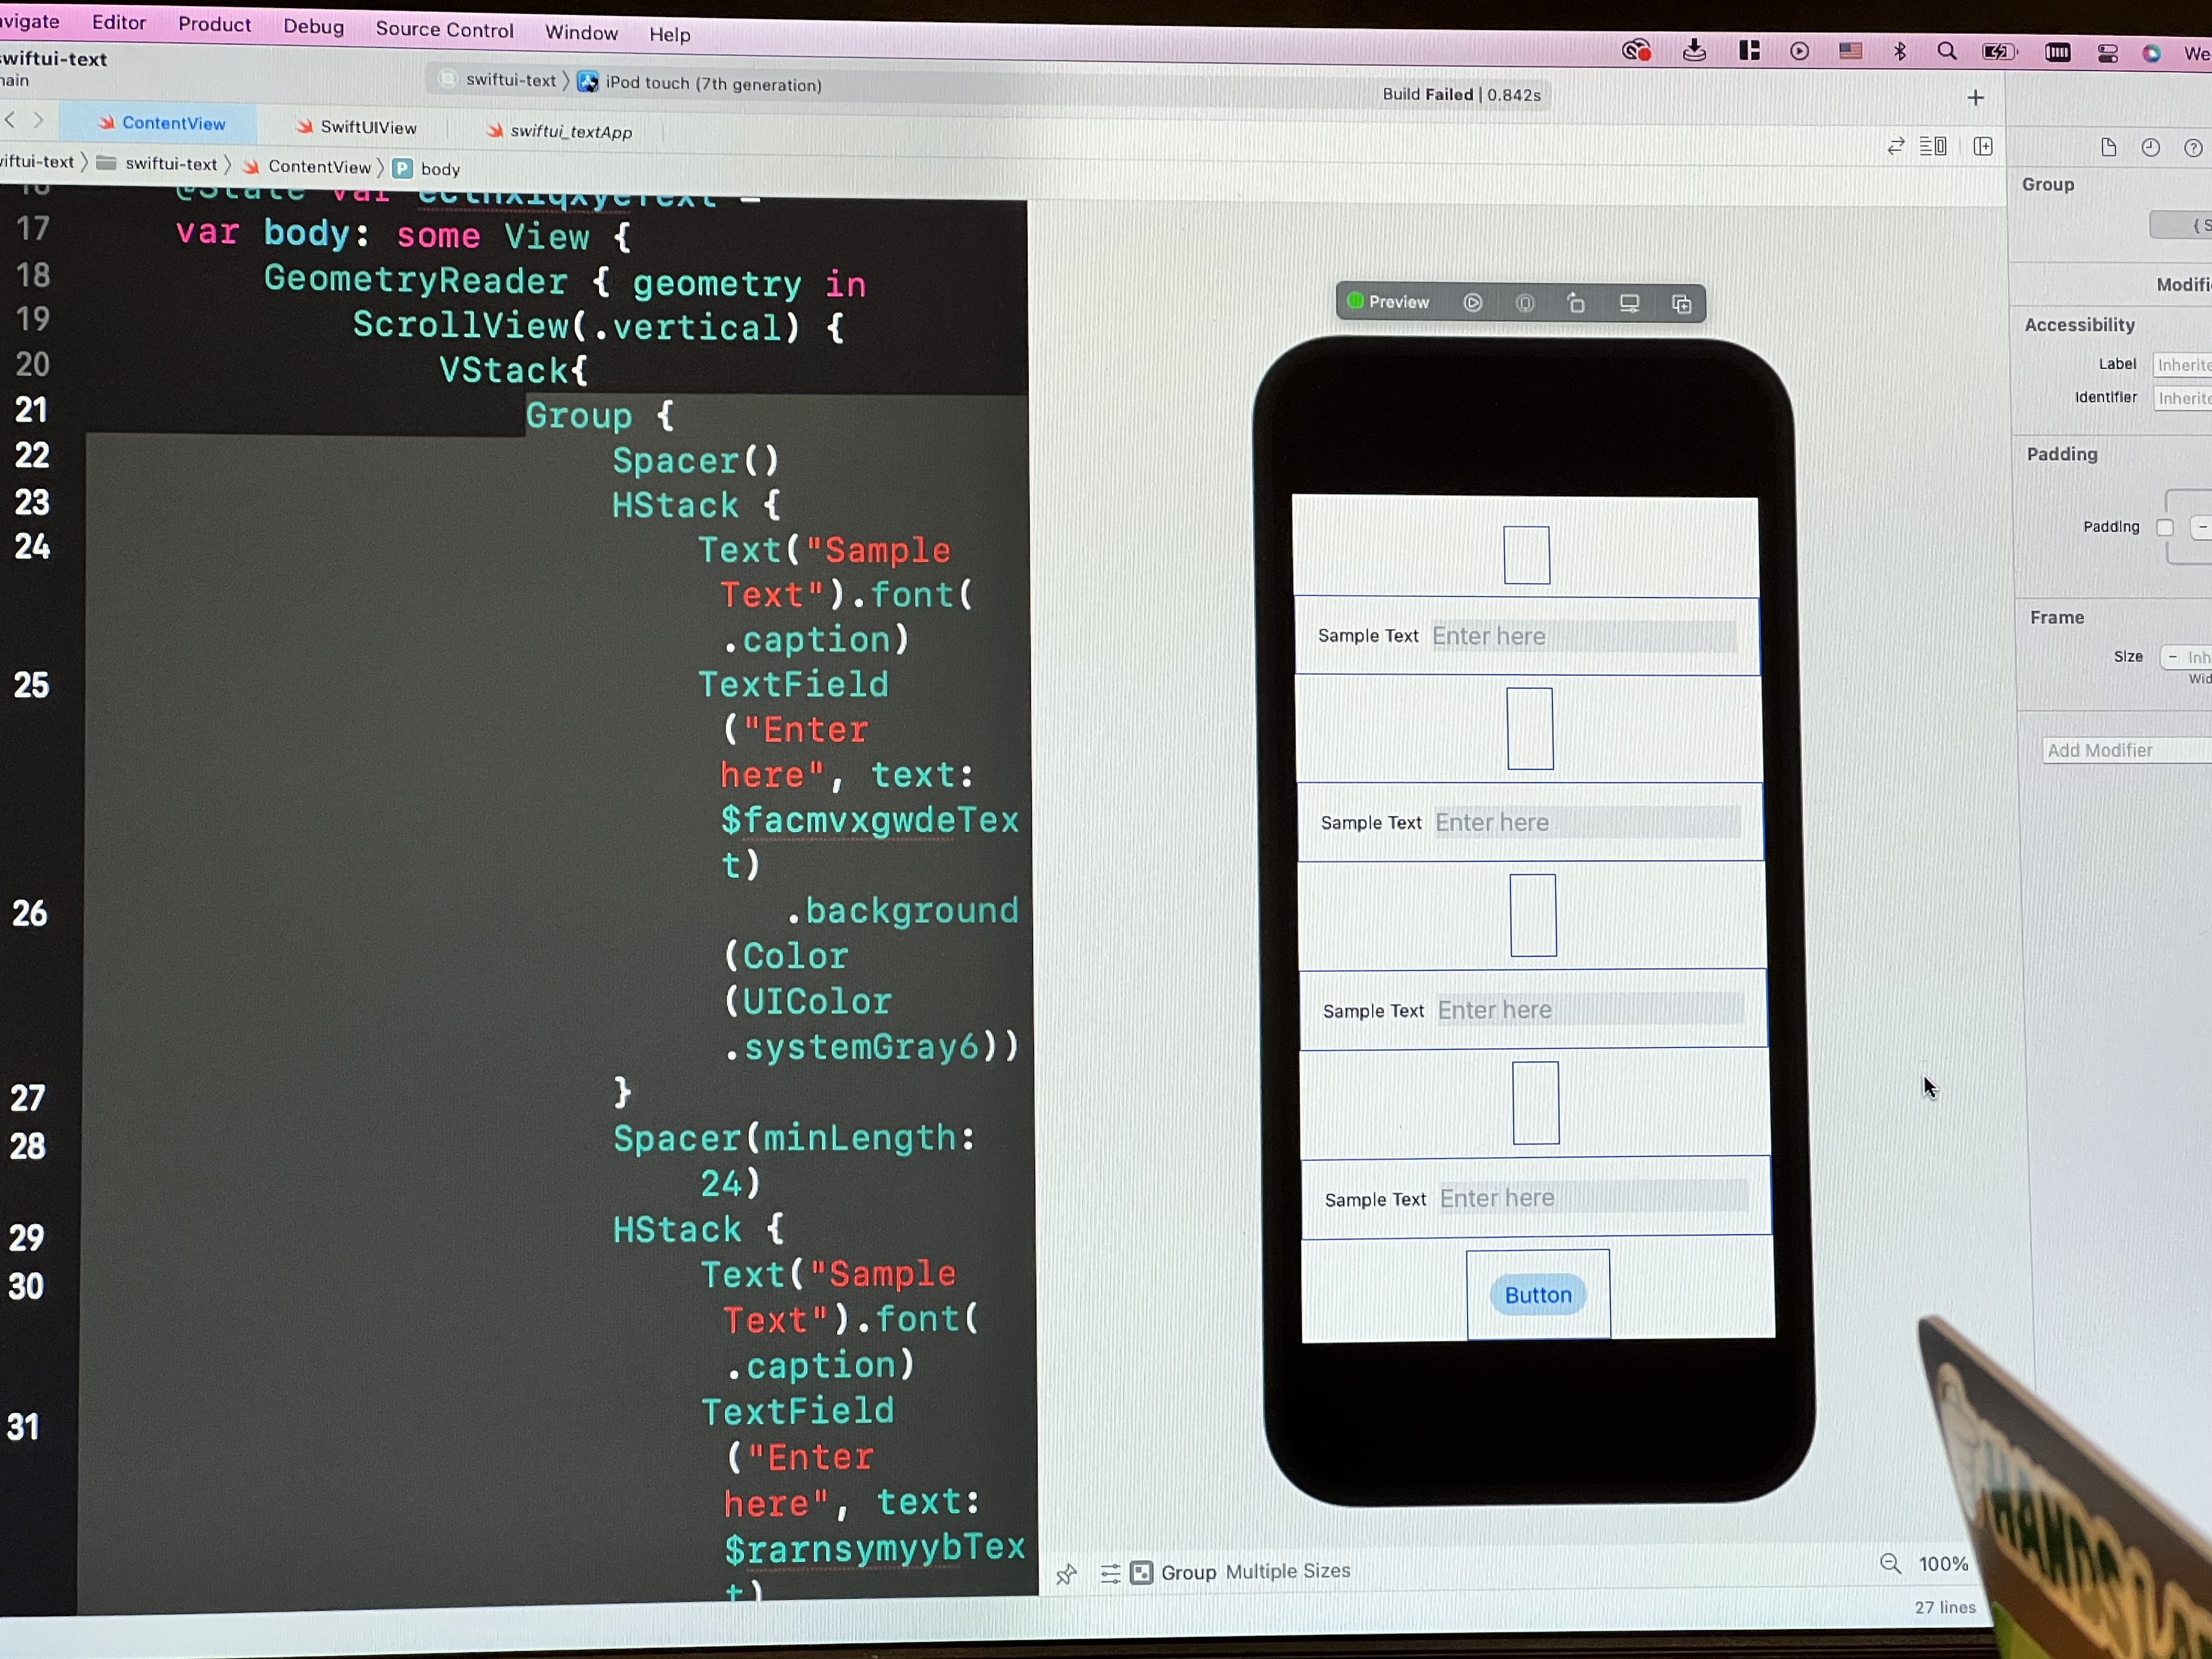
\includegraphics[width=100mm]{img/usertest_autogen_2.jpeg}
    \end{center}
    \caption{被験者B自動生成UI}
    \label{fig:usertest_autogen_2}
  \end{minipage}
\end{figure}


\begin{figure}[htbp]
  \begin{minipage}{\hsize}
    \begin{center}
       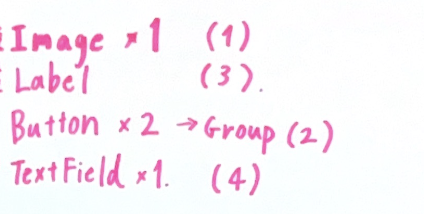
\includegraphics[width=50mm]{img/usertest_viewstructure_3.png}
    \end{center}
    \caption{被験者C記入用紙}
    \label{fig:usertest_viewstructure_3}
  \end{minipage}
\end{figure}

%\begin{figure}[htbp]
%  \begin{minipage}{\hsize}
%    \begin{center}
%       \includegraphics[width=100mm]{img/usertest_autogen_3.jpeg}
%    \end{center}
%    \caption{被験者C自動生成UI}
%    \label{fig:usertest_autogen_3}
%  \end{minipage}
%\end{figure}


\begin{figure}[htbp]
  \begin{minipage}{\hsize}
    \begin{center}
       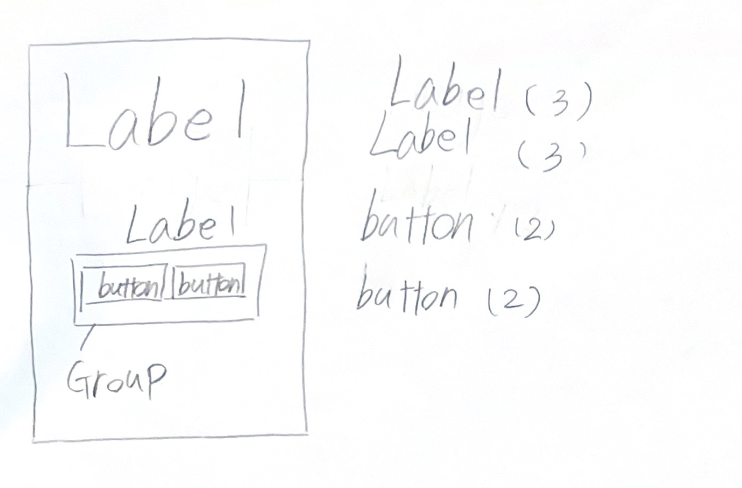
\includegraphics[width=50mm]{img/usertest_viewstructure_4.png}
    \end{center}
    \caption{被験者D記入用紙}
    \label{fig:usertest_viewstructure_4}
  \end{minipage}
\end{figure}

\begin{figure}[htbp]
  \begin{minipage}{\hsize}
    \begin{center}
       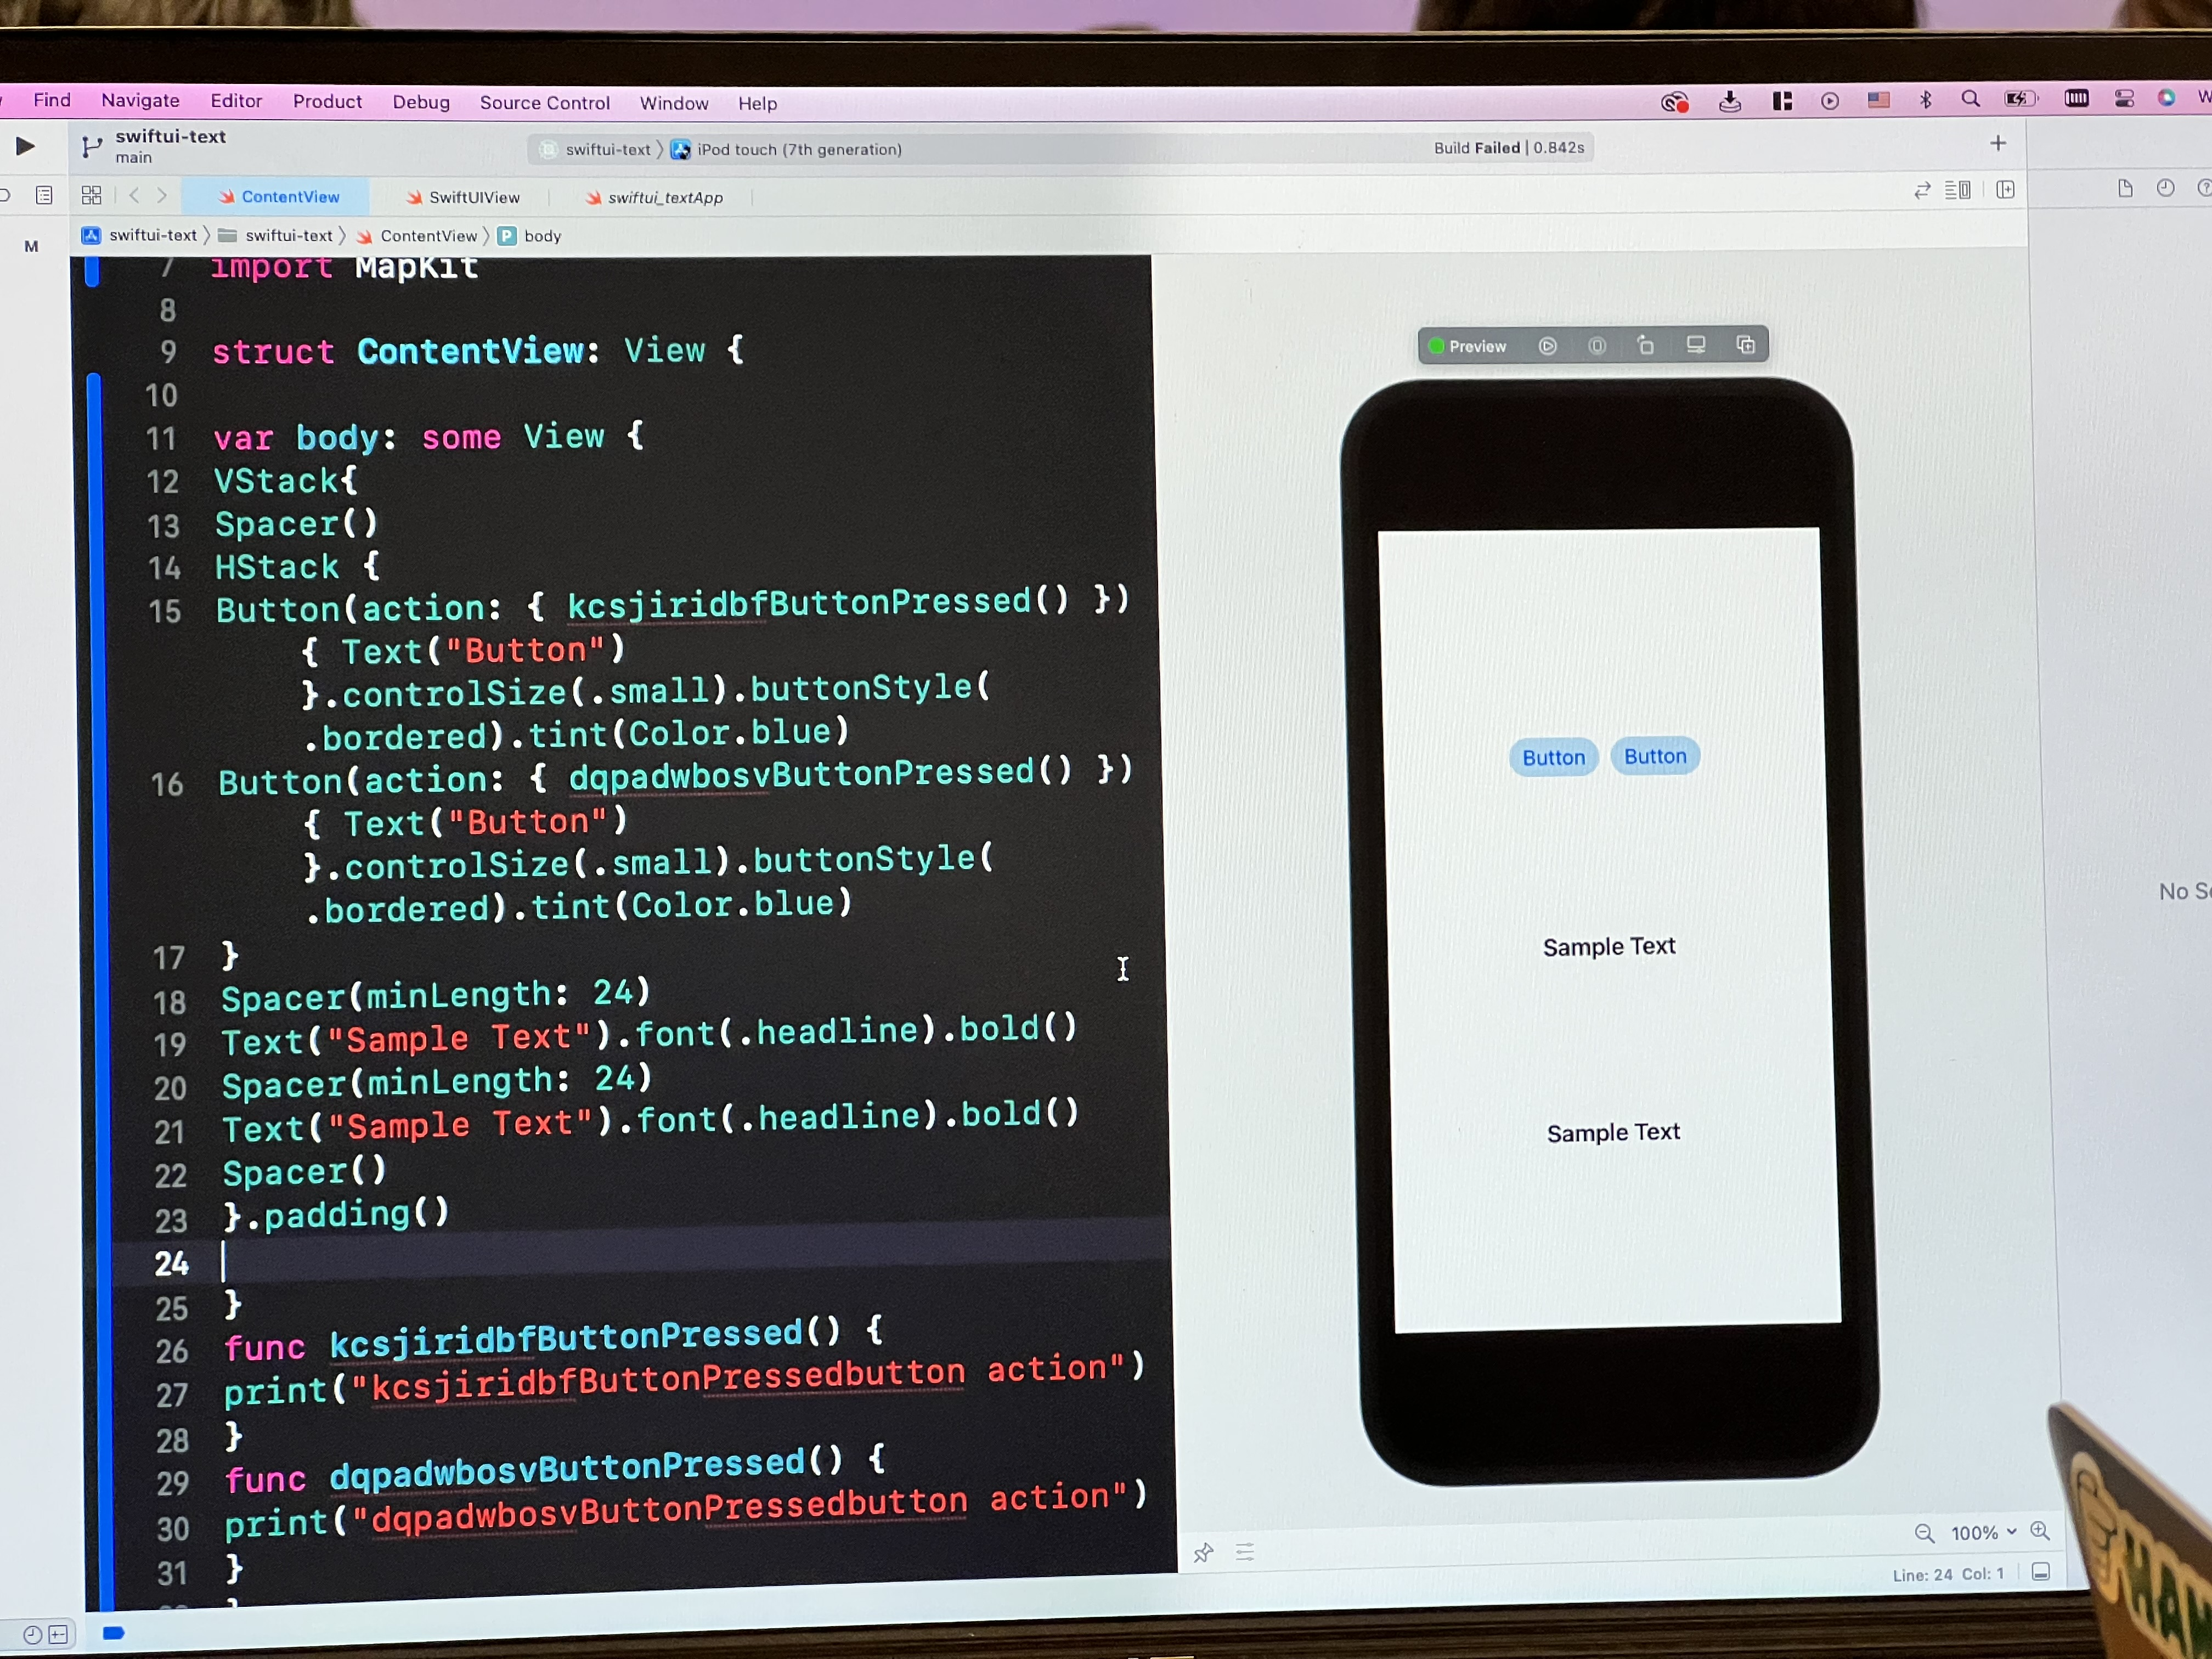
\includegraphics[width=100mm]{img/usertest_autogen_4.jpeg}
    \end{center}
    \caption{被験者D自動生成UI}
    \label{fig:usertest_autogen_4}
  \end{minipage}
\end{figure}


\begin{figure}[htbp]
  \begin{minipage}{\hsize}
    \begin{center}
       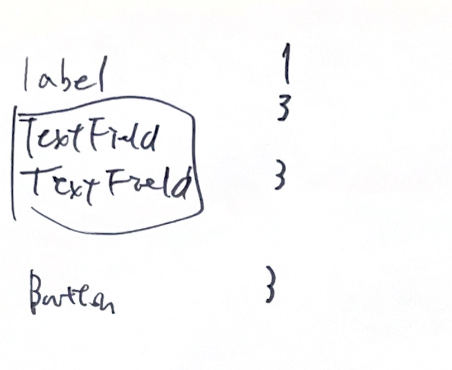
\includegraphics[width=50mm]{img/usertest_viewstructure_5.png}
    \end{center}
    \caption{被験者E記入用紙}
    \label{fig:usertest_viewstructure_5}
  \end{minipage}
\end{figure}

\begin{figure}[htbp]
  \begin{minipage}{\hsize}
    \begin{center}
       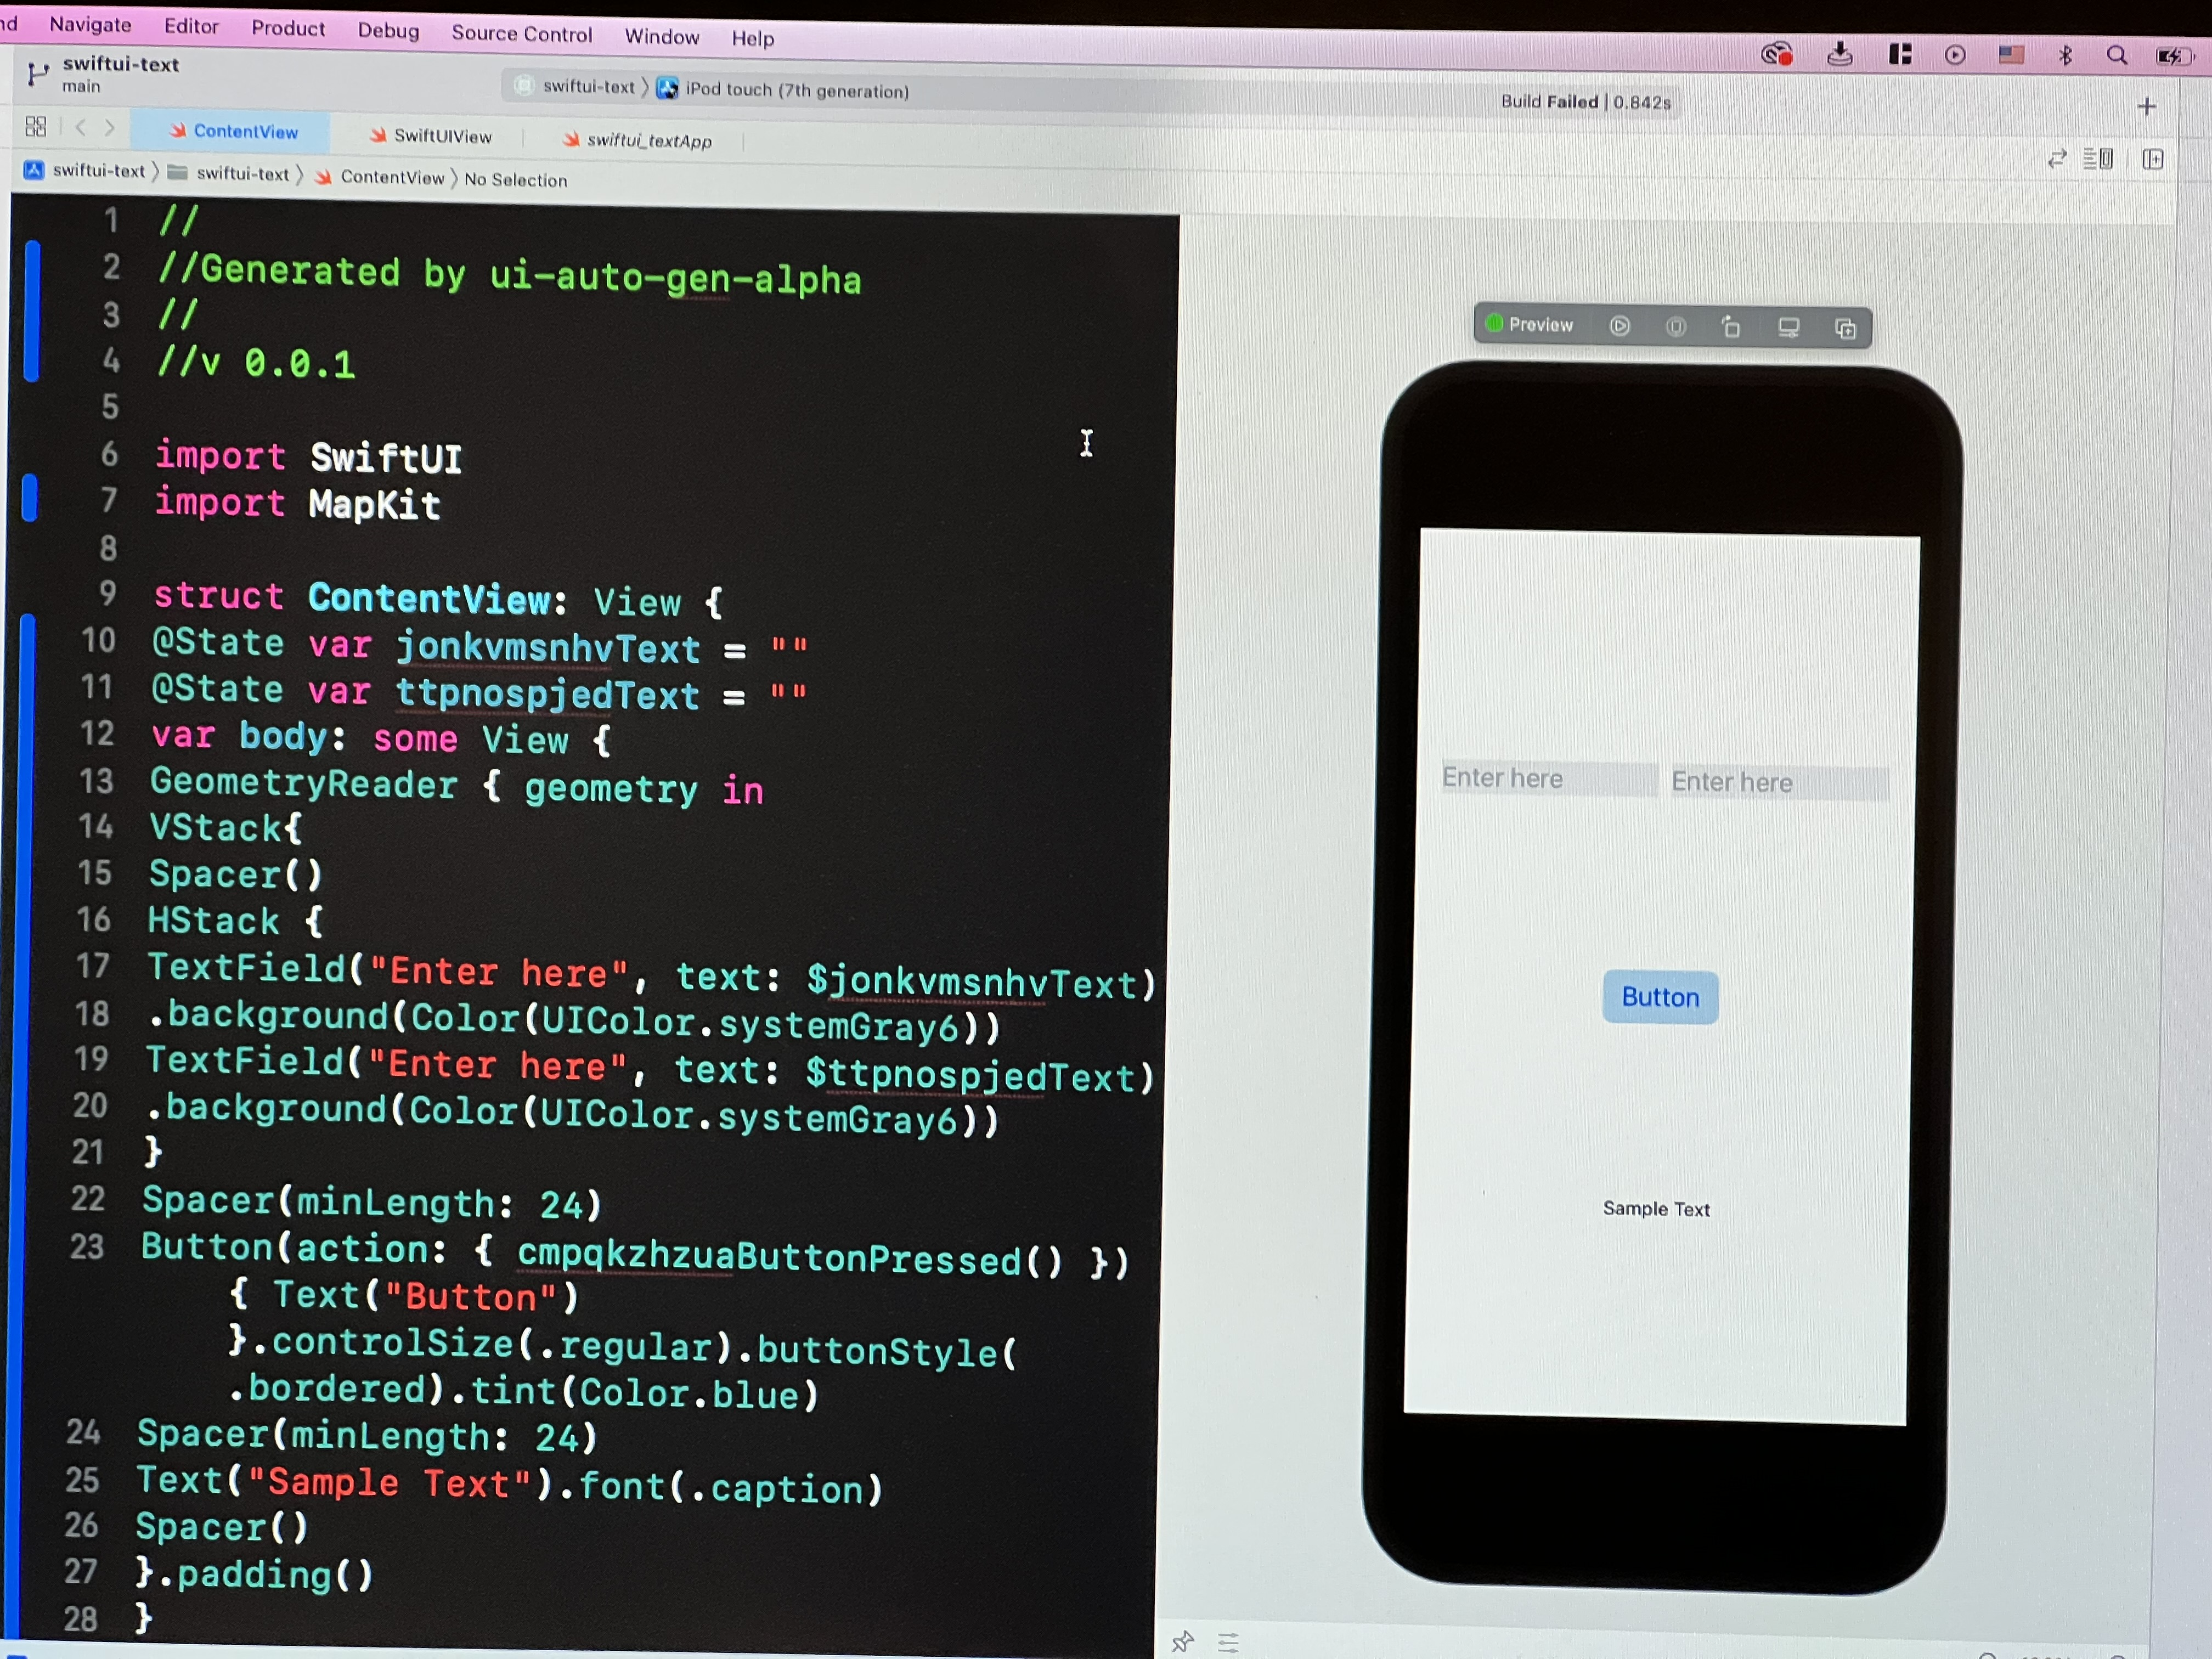
\includegraphics[width=100mm]{img/usertest_autogen_5-1.jpeg}
    \end{center}
    \caption{被験者E自動生成UI}
    \label{fig:usertest_autogen_5-1}
  \end{minipage}
\end{figure}

\begin{figure}[htbp]
  \begin{minipage}{\hsize}
    \begin{center}
       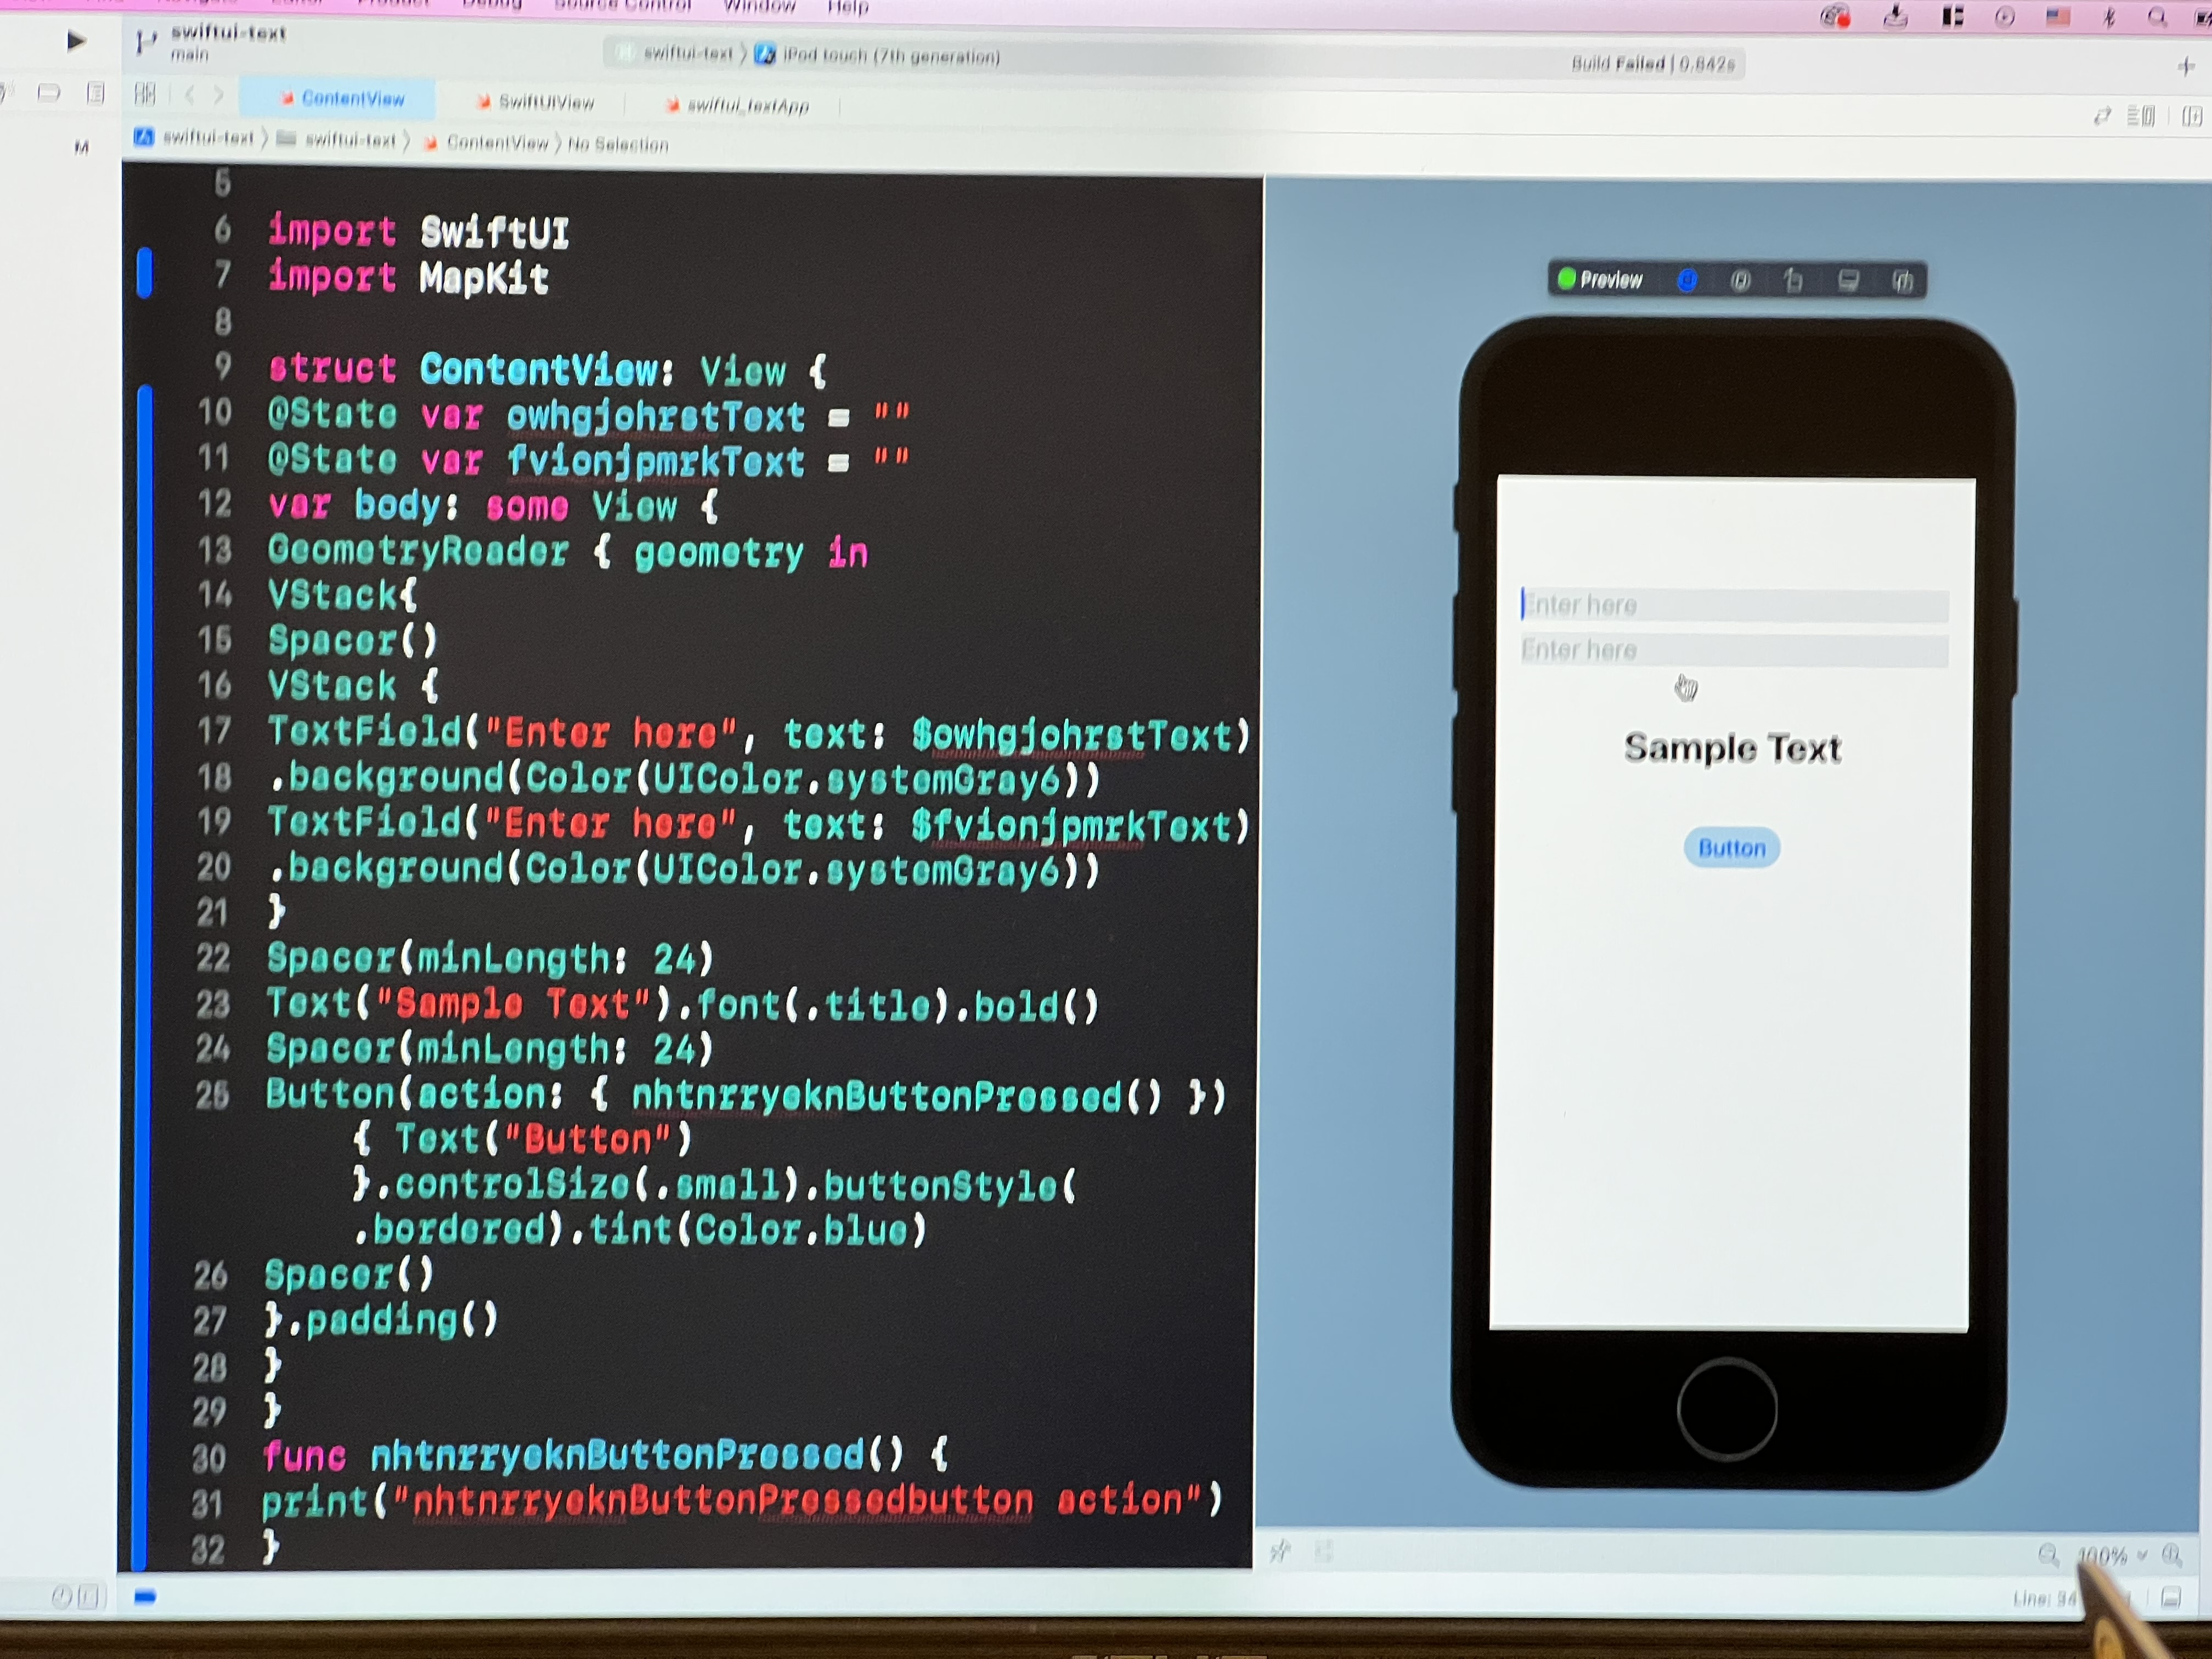
\includegraphics[width=100mm]{img/usertest_autogen_5-2.jpeg}
    \end{center}
    \caption{被験者E自動生成UI-2}
    \label{fig:usertest_autogen_5-2}
  \end{minipage}
\end{figure}



\subsection{結果と考察}
本実験を通して,既存UIを本システムで再現すること,ある程度アプリ開発について知識のある人なら本システムを利用してUIを生成することが可能であることが明らかになった.またアンケート結果によると(付録A, Bを参照)UIの生成を自動化することで効率化が図れることがわかった.

また普段デザインの見栄えを考えるあまりUIとしての本来の目的を見失いがちになるとの意見もあった.本システムはそのような場合にでも本来の目的に向かって進むことができるツールになり得る.

そしてUIの設計開発ではダークモード対応,多画面サイズ対応,アクセシビリティ対応等工数はかかるものの,単純な作業が必要である.この部分についてもアンケートで実装する上で大変だと思うことで回答されており,本自動生成システムを使用することで自動で実装されるため本システムはとても有用であるといえる.





















  % 本文4
\chapter{結論}
\label{chap:conclusion}

\section{満足性評価のための指標の提案}

\section{評価システムの提案}

\section{今後の課題}

  % 本文5

\begin{acknowledgment}

本論文の作成にあたり,研究室聴講時代から終始適切な助言を賜り,また丁寧に指導してくださった増井俊之教授に深く感謝申し上げます.増井俊之教授には本研究のみならず,日頃からプロダクト,アイディアに対してもNOTA CTOとしてのプロダクト開発の側面のご意見,研究者としての学術的なご意見を多数賜りました.感謝申し上げます.増井研究会では,博士課程の田中優氏,修士課程OBの左治木隆成氏には様々なご意見をいただき充実した研究会活動をさせていただきました.卒業生の皆様,研究会メンバーの民様にも多くのご支援をいただきました.

また同輩であり,孫正義育英財団\cite{masason} 正財団生であり,Bridge UI株式会社\cite{bridgeui}代表取締役社長兼CTOの佐々木雄司氏には気の置ける友人として,日々的確で新しい意見をいただいた他,\TeX の環境構築にも多大なるご支援をいただきました.

そして1年次よりデザインに関する終始適切な助言を賜り,丁寧に指導してくださった鳴川肇准教授に感謝申し上げます.また鳴川研究会メンバーの皆様にも日々たくさんのご支援をいただきました.

公私に渡りご指導,ご支援いただきました皆様に心から感謝申し上げます.
\begin{flushright}
2022年1月 吉日

尾崎 正和
\end{flushright}
\end{acknowledgment}
  % 謝辞。要独自コマンド、include先参照のこと

\begin{bib}[99]

\bibliography{main}

\end{bib}
  % 参考文献。要独自コマンド、include先参照のこと
\appendix
\chapter{UI自動生成システムユーザテスト 質問紙}
\begin{enumerate}
  \item 年齢
  \item 性別(Biological)
  \\選択肢
 \begin{itemize}
  \item 男性
  \item 女性
  \item その他
  \item 無回答
\end{itemize}
\item 普段アプリ開発において,デザインとはどのようなことをおこなっていますか.
\item 今回の自動システムを使った率直な感想をお願いします.
\item 優先度を調整して思い通りのUIに近づきましたか.
\item 普段UIを考える,実装する上で大変だと思うことは何ですか.
\item 全体を通しての感想や意見などなんでも記入してください.
\end{enumerate}

\chapter{UI自動生成システムユーザテスト 記述解答}

\section{普段アプリ開発において,デザインとはどのようなことをおこなっていますか.}
\begin{itemize}
	\item 色々なモチーフを組み合わせてSketchやイラレに書き起こす
	\item テーマを決めて統一させる、パーツを置いてみる、色合いを見る
	\item 載せたい内容を一度整理する。
	\item PinterestでUIのデザインを調べたり、友だちや家族にUIのデザインの案を見てもらい、どうしたら、もっと見やすくなるかなどを聞いて、より使いやすいUIのデザイン考えています。
	\item ラフスケッチ、ワイヤーフレームを作ってみたりして、ユーザーに見せたい順番で、文字の大きさや配置を考えてどの順番で追っていくかを考える
\end{itemize}

\section{今回の自動システムを使った率直な感想をお願いします.}
\begin{itemize}
	\item すげぇ!!デザインするとき時短になりそう
	\item 自分でやらないといけないことが自動でできて嬉しかった
	\item 画期的で素晴らしいと思いました。
	\item UIのデザインを考えるとき、かなり悩むので、悩まなくてよくなるのは、とても便利だと思いました。
	\item UIパーツと優先順位の数の二つを決めるだけで実装できるようになるのが簡単で普段時間がかかる実装も試しやすかった
\end{itemize}

\section{優先度を調整して思い通りのUIに近づきましたか.}
\begin{itemize}
	\item 近づいた
	\item 近づいた
	\item 近づいた。
	\item 近づいた!!優先順位を決めるだけで大きさを勝手に調節してくれるから、デザインに悩む時間が減って実装しやすくなると思った!!
	\item 近づきました。
\end{itemize}

\section{普段UIを考える,実装する上で大変だと思うことは何ですか.}
\begin{itemize}
	\item バランス、押しやすいボタンの幅を考えたりすること
	\item パーツの場所を考える、コンセプト?を決める
	\item デザインの見栄えを考えるあまり、UIとしての本来の目的を見失いがち。
	\item どのようなUIが直感的に使えるか、どうしたら見やすくなるかを考えている。考えたデザインをどうやってダークモードとライトモードに対応させるかが大変だと思っている。
	\item AutoLayoutを調節したり、配置したりすることが大変

\end{itemize}

\section{全体を通しての感想や意見などなんでも記入してください.}
\begin{itemize}
	\item AutoLayoutが楽になりそう!みんなが使ってハッカソンで同じUIが揃うの想像したら面白い
	\item コードを書かなくて済んで嬉しい
	\item 情報の優先度と載せる情報を整理して、デザインを考える過程を楽にできるので、UI構成の効率性を図ることができると思います。
	\item UIを作るときに、オートレイアウトを設定するのが面倒くさいので、優先順位をつけるだけで見やすいUIになるのはとても画期的だと思った。
	\item 簡単に実装できるようになるのが楽しくてこれから使えるようになったら、どんどん使ってみたい!
\end{itemize}    % 付録

\end{document}
